\documentclass[11pt,oneside]{memoir-article}
\usepackage{local}
\renewcommand{\docVersion}{v1.3.1}
\renewcommand{\docUrl}{\href{https://github.com/profound-labs/wallcalendar/}{link}}
\hypersetup{ pdfauthor={Gambhīro Bhikkhu}, }
\author{Gambhīro Bhikkhu}
\date{\today}
\title{Wallcalendar User Manual}
\hypersetup{
 pdfauthor={Gambhīro Bhikkhu},
 pdftitle={Wallcalendar User Manual},
 pdfkeywords={},
 pdfsubject={},
 pdfcreator={Emacs 25.1.1 (Org mode 9.0.9)}, 
 pdflang={English}}
\begin{document}

\maketitle
\bigskip

\thispagestyle{empty}

This is the \textbf{User Manual} for the \texttt{wallcalendar} class.
\textbf{Source documentation} is in \texttt{wallcalendar-code.pdf}. Clone or
download from Github:

\href{https://github.com/profound-labs/wallcalendar/}{https://github.com/profound-labs/wallcalendar/}

The documentclass comes with the following layouts:

\bigskip

\makeatletter
\newlength\exampleWidth
\setlength{\exampleWidth}{45mm}
\makeatother

\begin{extrafullwidth}

\hfill
\begin{minipage}{0.31\linewidth}
\centering

Full page photo, the calendar days\\
overlaid with opacity

\bigskip

\frame{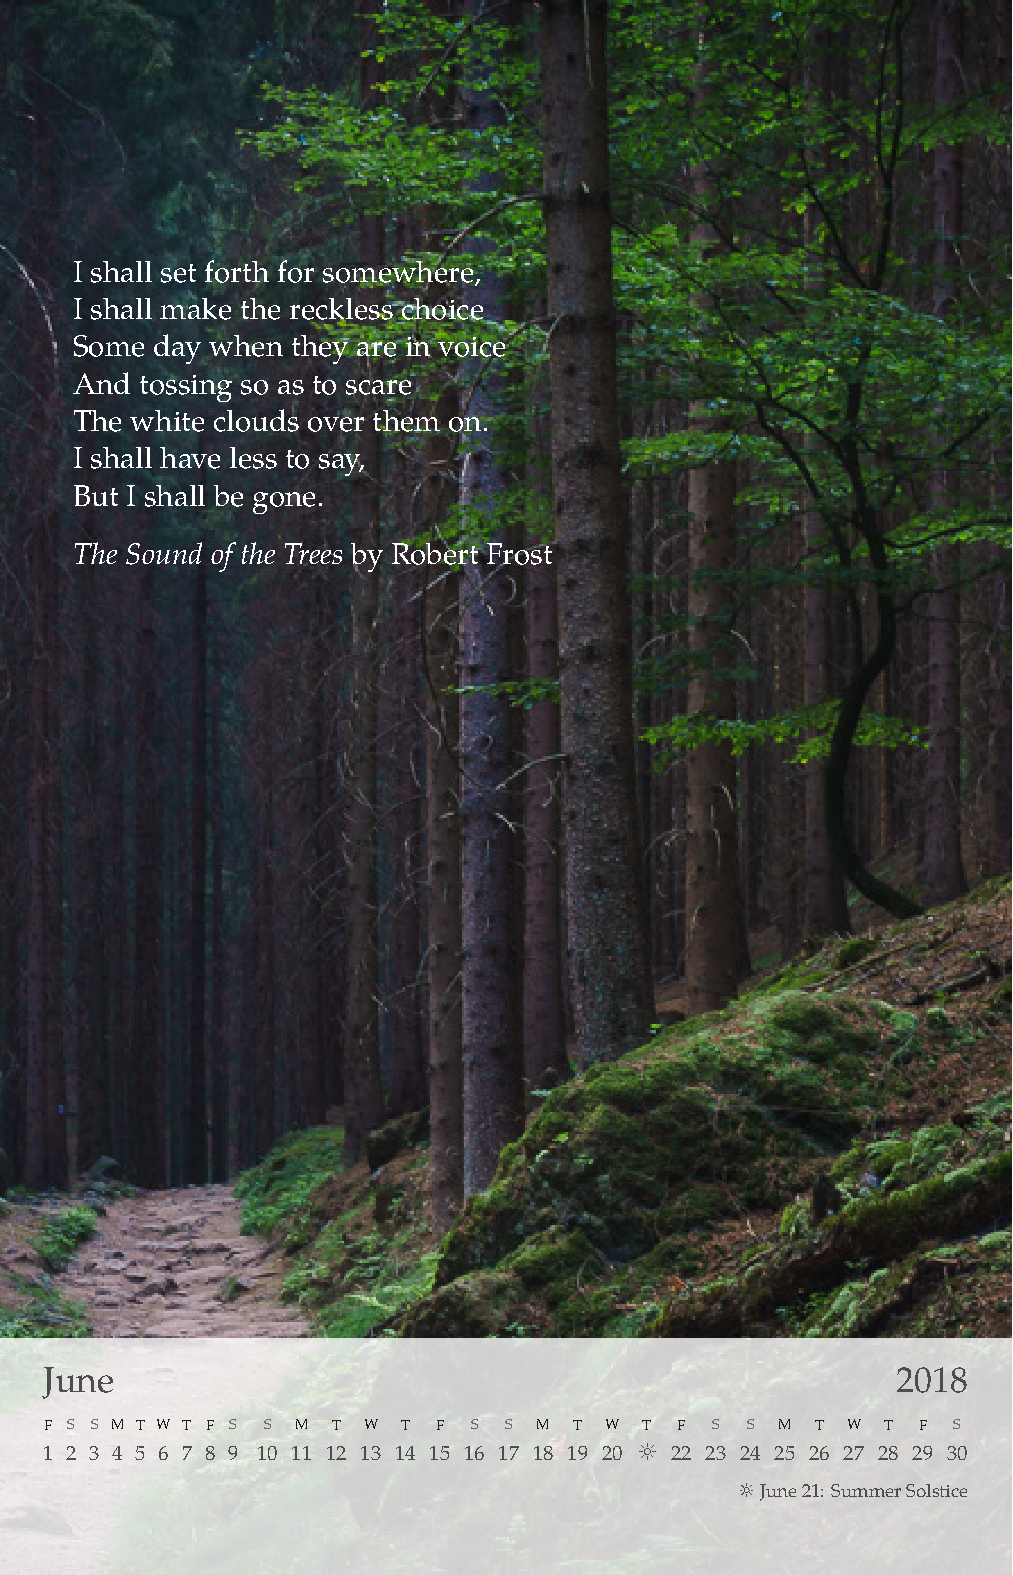
\includegraphics[width=\exampleWidth]{cal-plain-01}}

\end{minipage}%
\begin{minipage}{0.31\linewidth}
\centering

Full page photo, the photo above\\
the calendar days

\bigskip

\frame{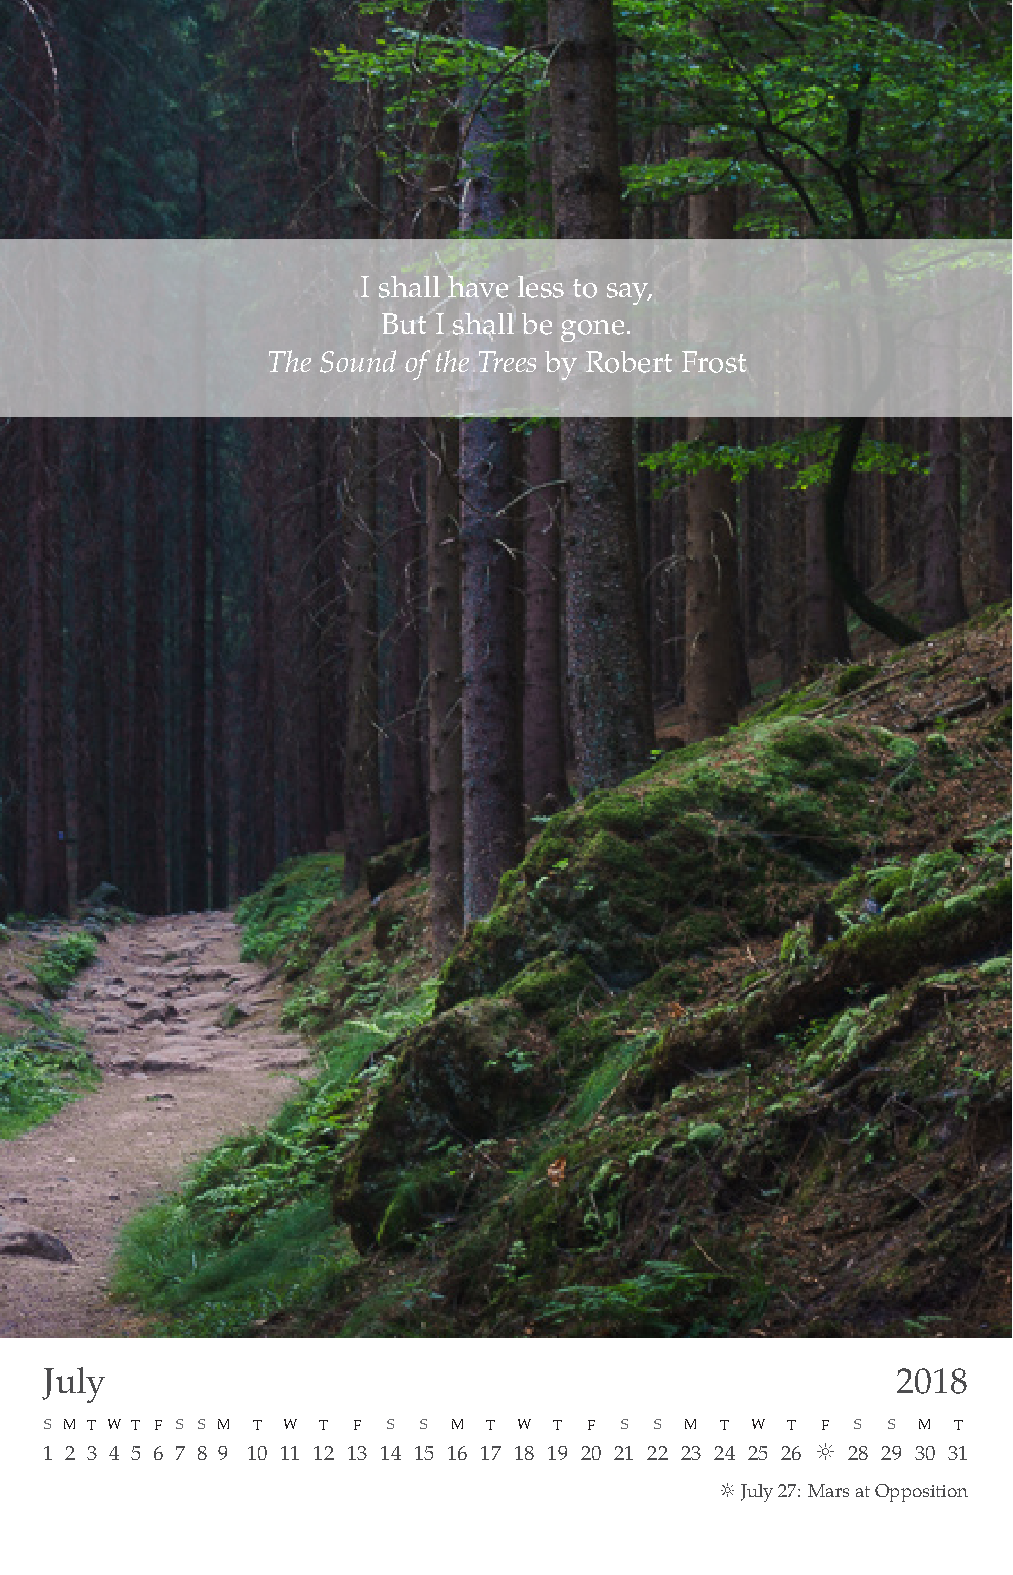
\includegraphics[width=\exampleWidth]{cal-plain-02}}

\end{minipage}%
\begin{minipage}{0.31\linewidth}
\centering

Small landscape photo, with a\\
calendar grid

\bigskip

\frame{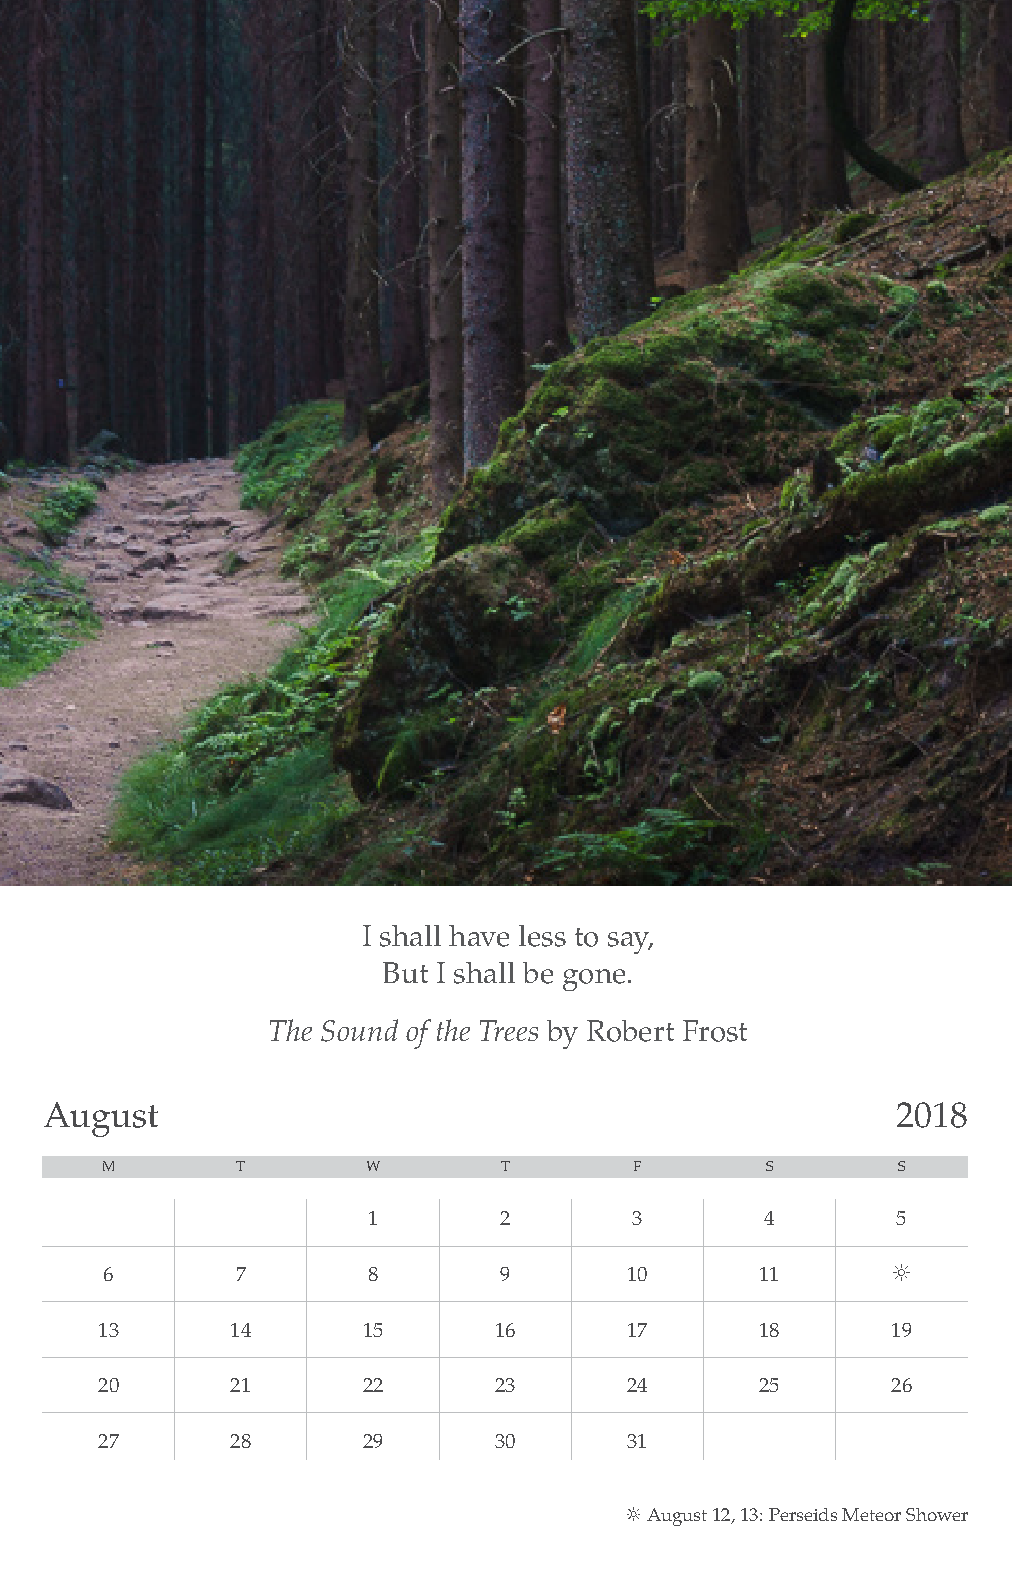
\includegraphics[width=\exampleWidth]{cal-plain-03}}

\end{minipage}
\hfill\mbox{}

\end{extrafullwidth}

\bigskip

\begin{extrafullwidth}

\hfill
\begin{minipage}{0.31\linewidth}
\centering

Load event marks from CSV file

\bigskip

\frame{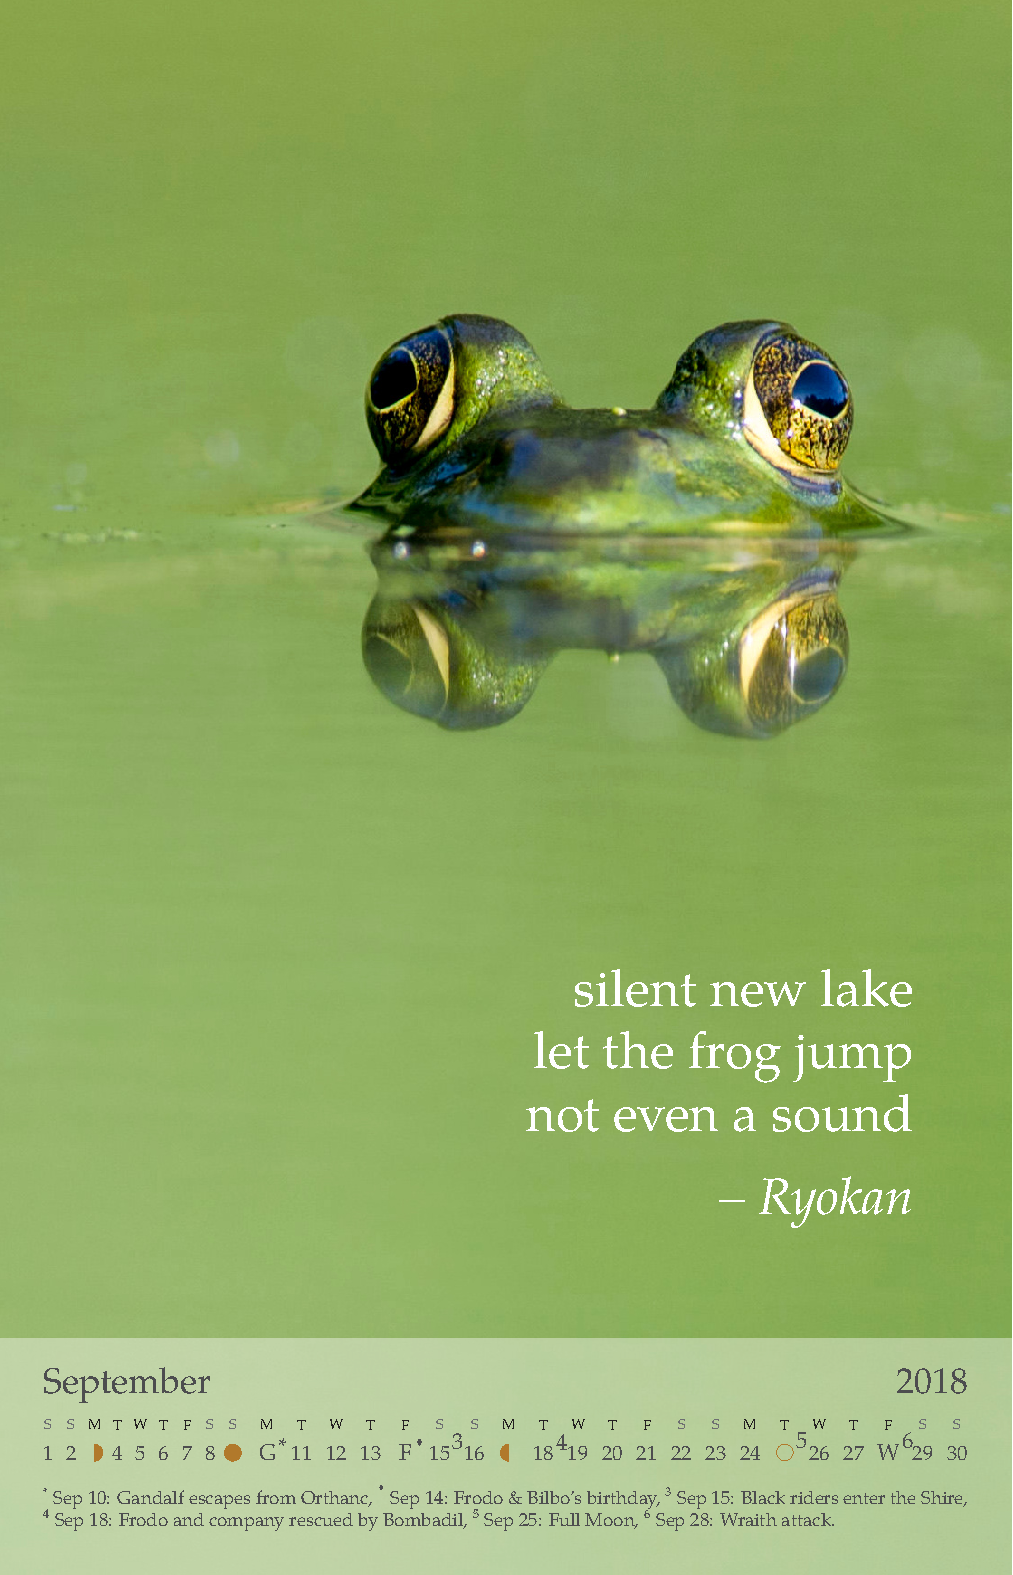
\includegraphics[width=\exampleWidth]{./examples/cal-marks.pdf}}

\end{minipage}%
\begin{minipage}{0.31\linewidth}
\centering

Year planner

\bigskip

\frame{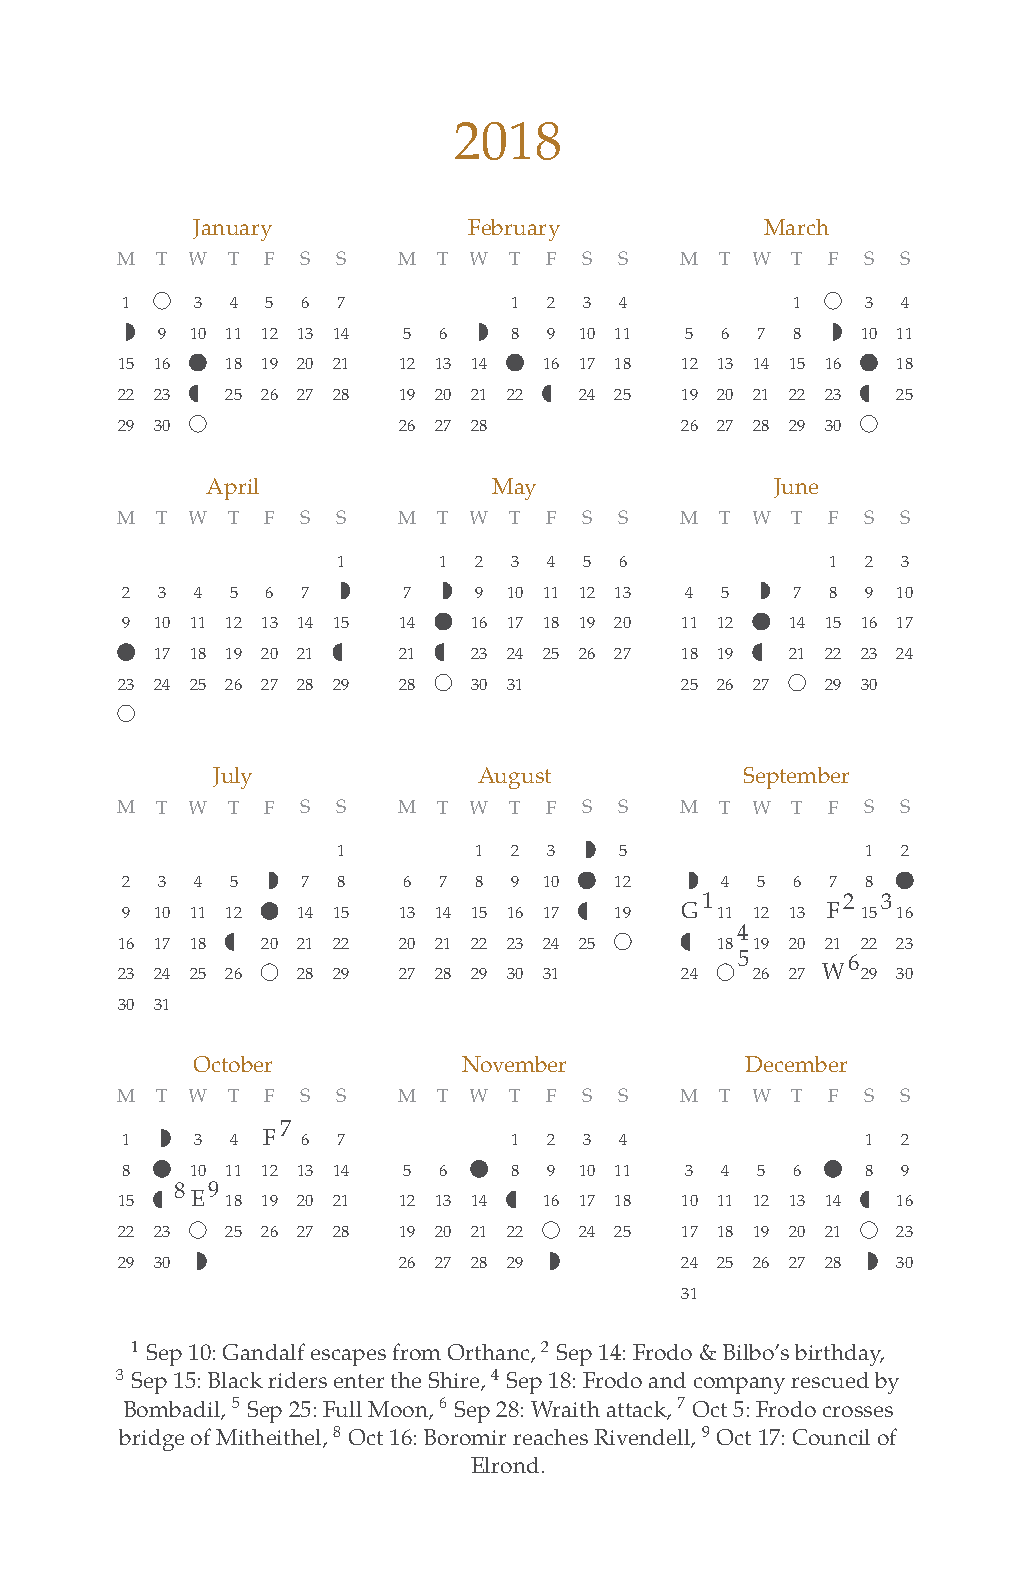
\includegraphics[width=\exampleWidth]{./examples/cal-year-planner.pdf}}

\end{minipage}%
\begin{minipage}{0.31\linewidth}
\centering

Thumbnails and captions

\bigskip

\frame{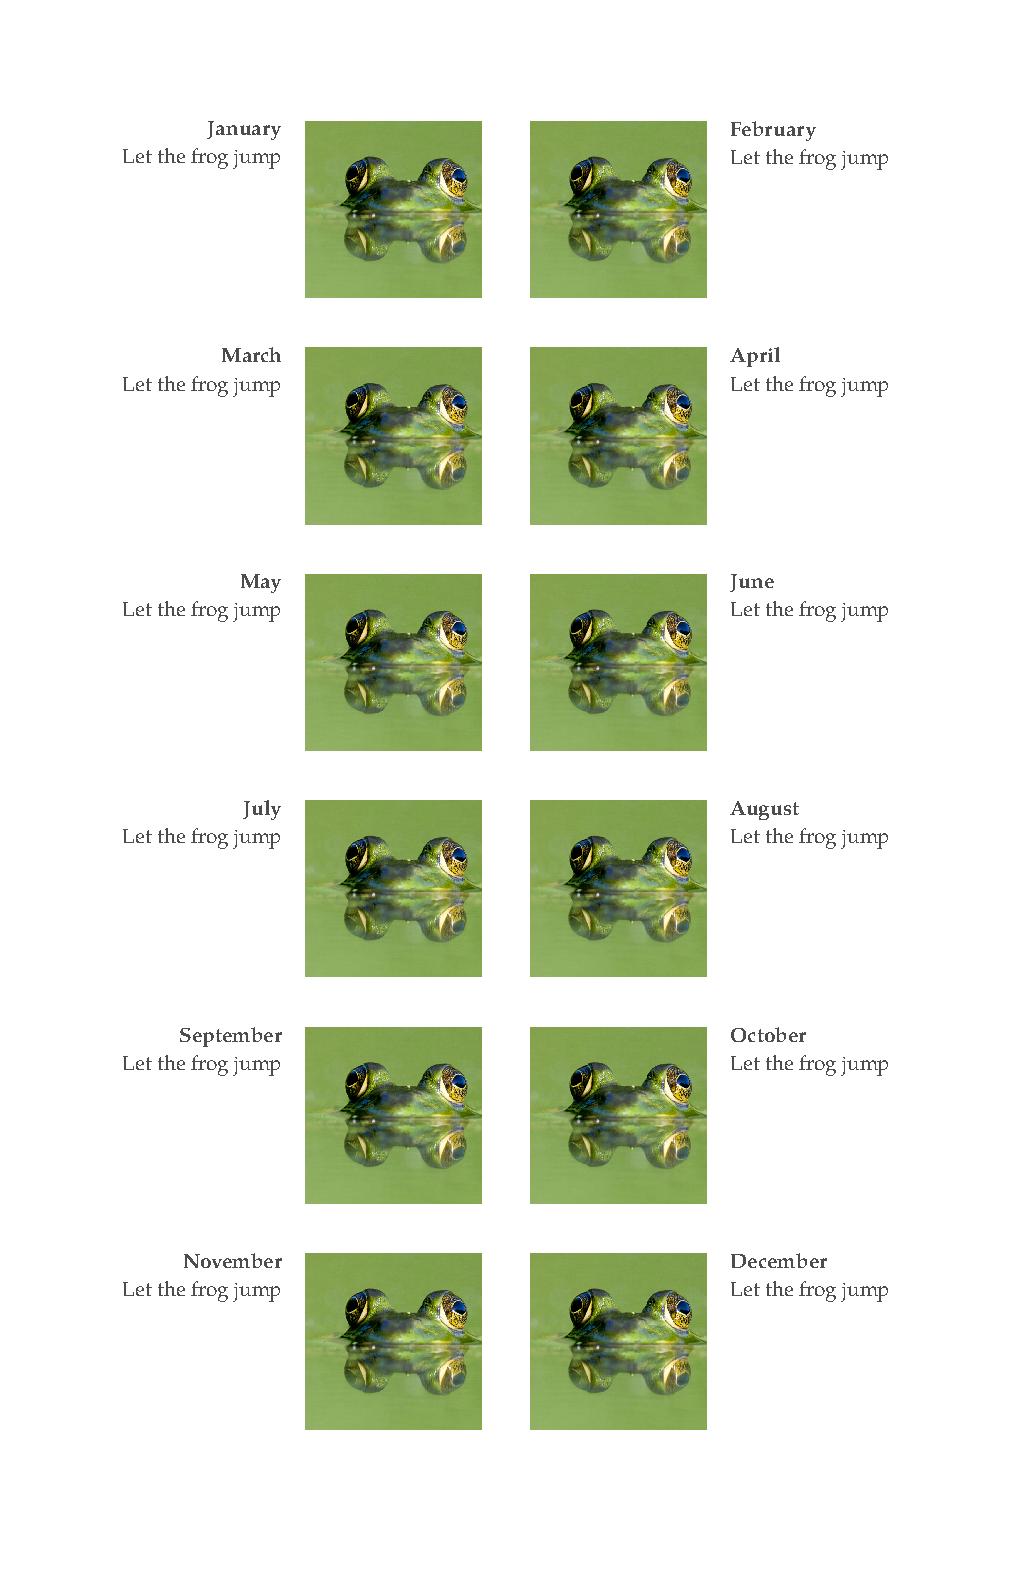
\includegraphics[width=\exampleWidth]{./examples/cal-thumbnails.pdf}}

\end{minipage}
\hfill\mbox{}

\end{extrafullwidth}

\clearpage

\tableofcontents*
\clearpage



\chapter{Tutorial: Forest Calendar}
\label{sec:org9e1c3d1}

In this tutorial we will produce the three example pages seen in the summary.

Set the parameters of the month pages in advance, either in the preamble or in
the document body, but before calling \texttt{\textbackslash{}MonthPage\{ month \}} to typeset it.

A month page can have four areas:

\begin{itemize}
\item Photo
\item Quote
\item Calendar
\item Events
\end{itemize}

Their parameters are set separately for each month:

\begin{verbatim}
\SetPhoto[ options ]{ month }
\SetQuote[ options ]{ month }{ quote text }
\SetCalendar[ options ]{ month }
\SetEvents[ options ]{ month }{ calendar tikz marks }{ events text }
\end{verbatim}

The month page will be typeset with:

\begin{verbatim}
\MonthPage[ options ]{ month }
\end{verbatim}

\section{Documentclass}
\label{sec:orgbba6dea}

To start, load the documentclass and set \texttt{year}, \texttt{language} and the \texttt{imageFolder}:

\begin{verbatim}
\documentclass[
  year=2018,
  language=english,
  imageFolder=./photos/,
]{wallcalendar}
\end{verbatim}

Let's start the preamble with \texttt{\textbackslash{}makeatletter} to be safe.

\begin{verbatim}
\makeatletter
\end{verbatim}

\section{Font settings}
\label{sec:org30e28c2}

For this example we'll use \TeX{} Gyre Pagella as the main typeface. We also load
DejaVu Sans to use a particular glyph as a mark in the calendar (\texttt{U+263C} white
sun with rays).

\begin{verbatim}
\usepackage{fontspec}
\defaultfontfeatures{Ligatures={TeX}}
\setmainfont{TeX Gyre Pagella}
\newfontfamily\dejaVuSans{DejaVu Sans}
\end{verbatim}

\clearpage

\section{June}
\label{sec:org6815f95}

\twocol{%
  \frame{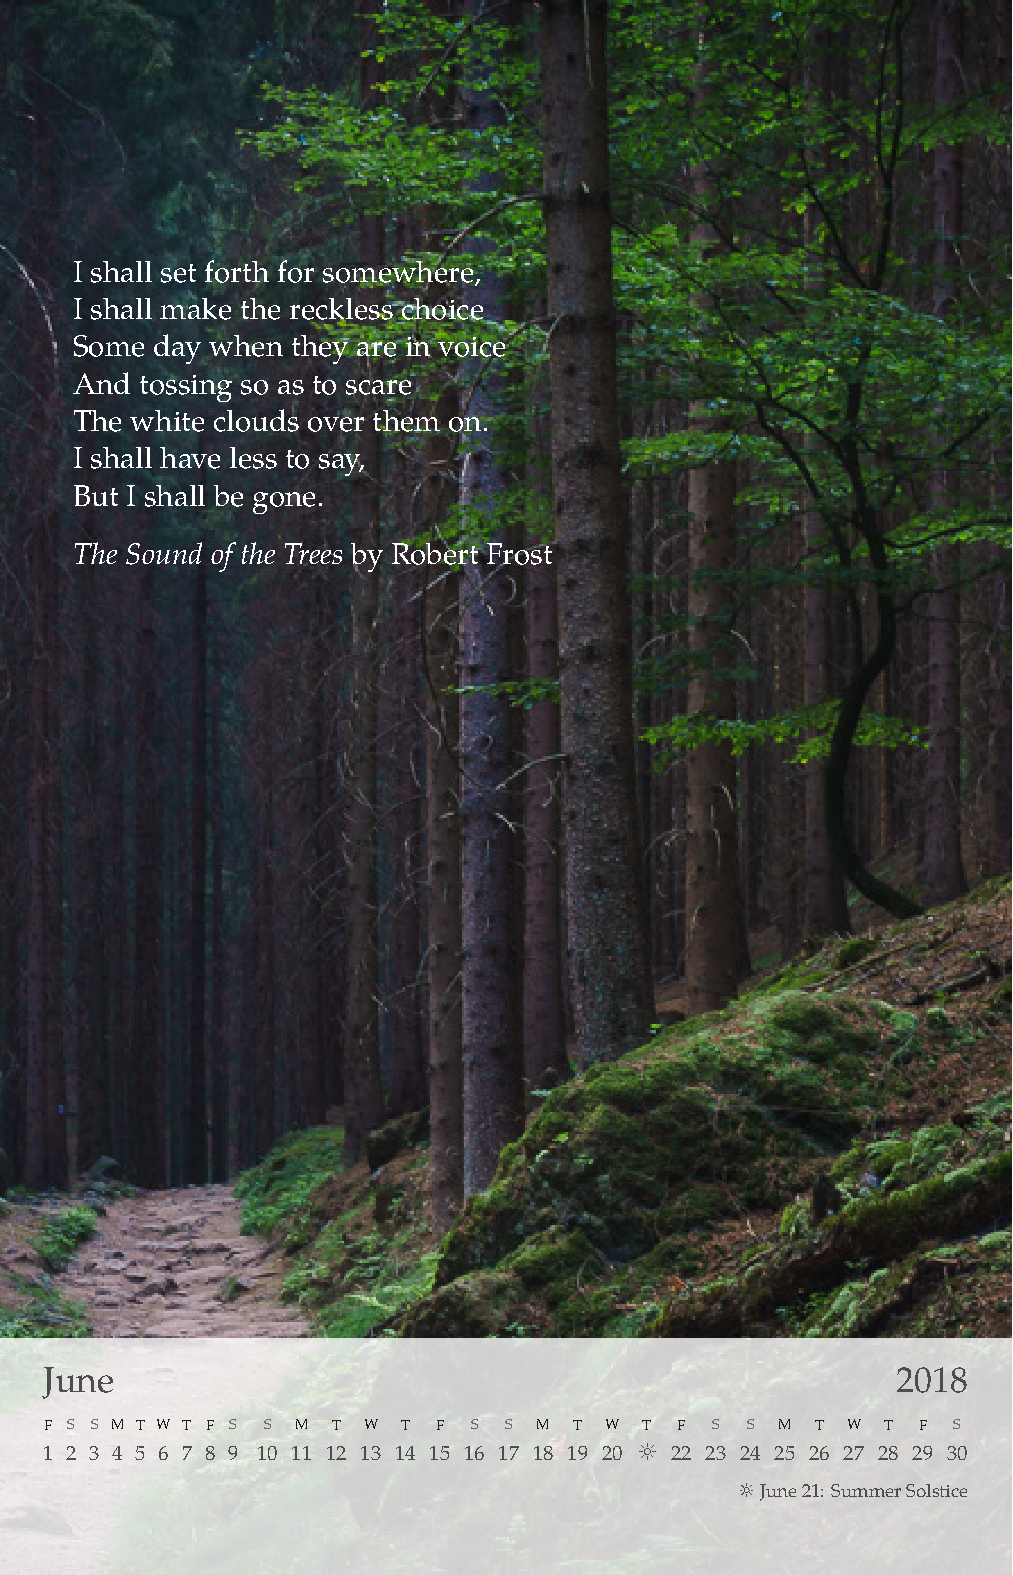
\includegraphics[width=5cm]{cal-plain-01}}%
}{%
  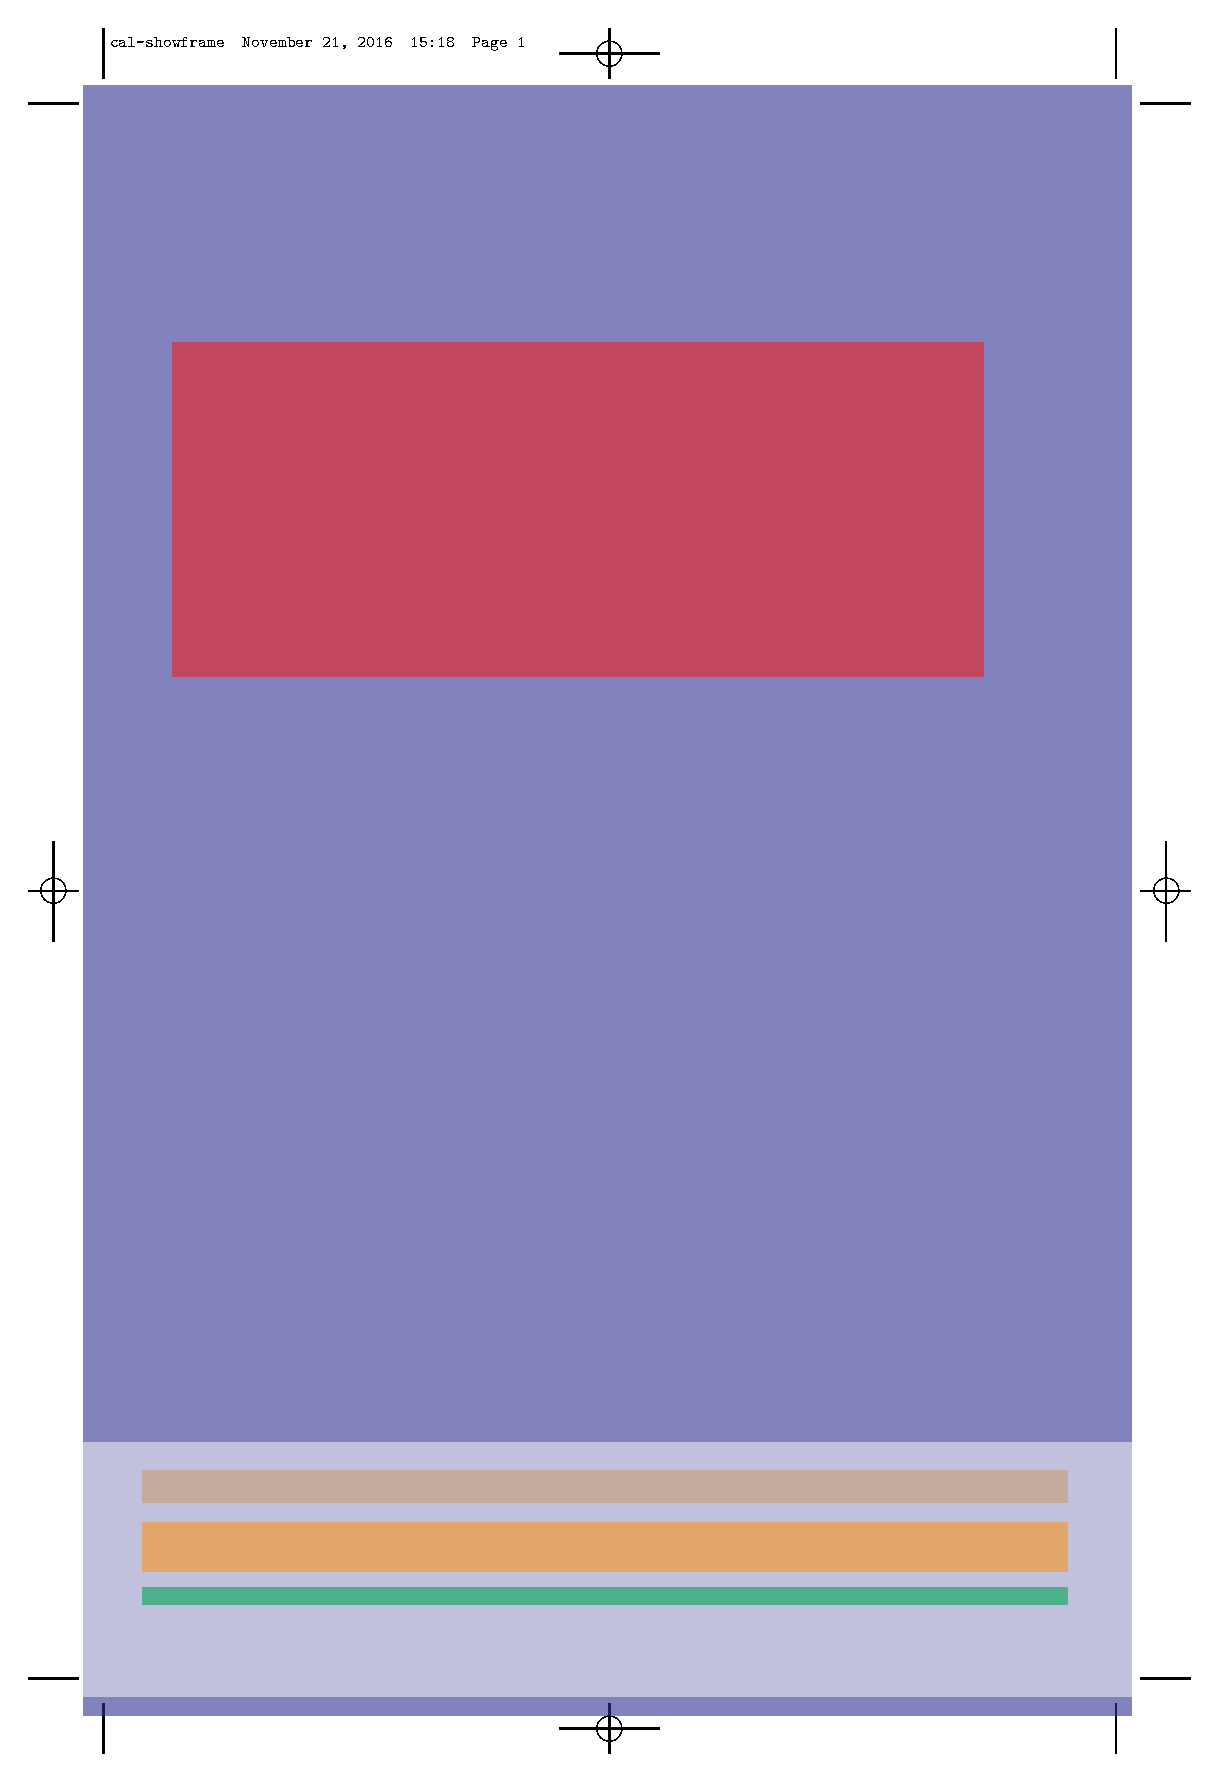
\includegraphics[width=6.12cm]{cal-showframe-01}%
}

\twocolcaption{\mbox{}}{%
  \raggedright
  \texttt{showtrims} and \texttt{showframe} class options show the page structure.
}

\bigskip

It will be a full page photo, with 3mm bleed on all four sides. You can see the
bleed if you enable the \texttt{showtrims} class option. We also specify the file name
of the photo (no extension), this will be the argument of \texttt{\textbackslash{}includegraphics}.

\begin{verbatim}
\SetPhoto[bleed=3mm, file={obscure-crop}]{June}
\end{verbatim}

A quote will be positioned over the photo. The quote is in a \texttt{\textbackslash{}linewidth} wide
minipage, attached to the top left corner of the page. Use \texttt{\textbackslash{}raggedleft},
\texttt{\textbackslash{}raggedright}, or \texttt{\textbackslash{}centering} for alignment, and the \texttt{xOffset} and \texttt{yOffset}
options to move the quote's minipage to the exact position.

\begin{verbatim}
\SetQuote[xOffset=-5mm, yOffset=-20mm]{June}{%
\raggedright
\setlength{\parskip}{10pt}%
\Large
\color{white}

I shall set forth for somewhere,\\
I shall make the reckless choice\\
Some day when they are in voice\\
And tossing so as to scare\\
The white clouds over them on.\\
I shall have less to say,\\
But I shall be gone.

\textit{The Sound of the Trees} by Robert Frost
}
\end{verbatim}

The layout macro will place the calendar at the bottom, dates in a single line.

Here we use a conditional to use a different calendar style when \texttt{showframe} is
turned on, this helps with debugging or tuning the position.

\begin{verbatim}
\ifshowframe
  \SetCalendar[bg/.style={opacity=0.5, fill=white}]{June}
\else
  \SetCalendar[bg/.style={opacity=0.8}]{June}
\fi
\end{verbatim}

Events for particular days are printed under the calendar.

\begin{verbatim}
\SetEvents{June}{%
  if (equals=2018-06-21)
    [day text={\dejaVuSans\char"263C}];% U+263C white sun with rays
}{%
\raggedleft
{\dejaVuSans\char"263C} June 21: Summer Solstice
}
\end{verbatim}

\section{July}
\label{sec:orgda955cc}

\twocol{%
  \frame{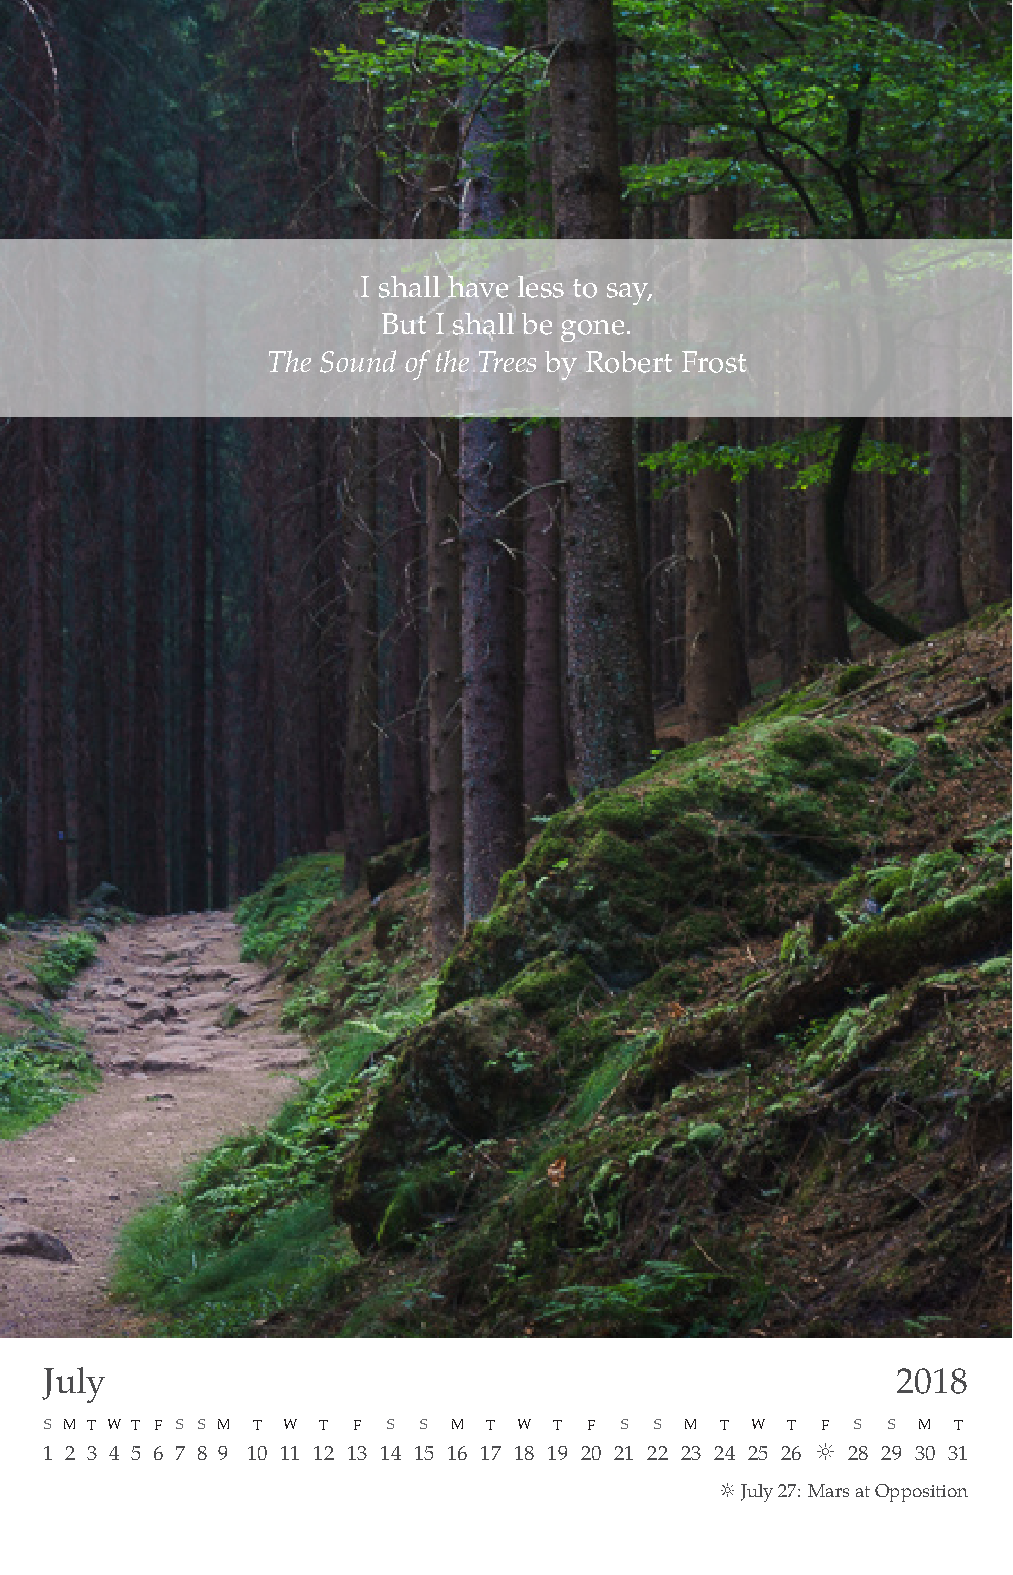
\includegraphics[width=5cm]{cal-plain-02}}%
}{%
  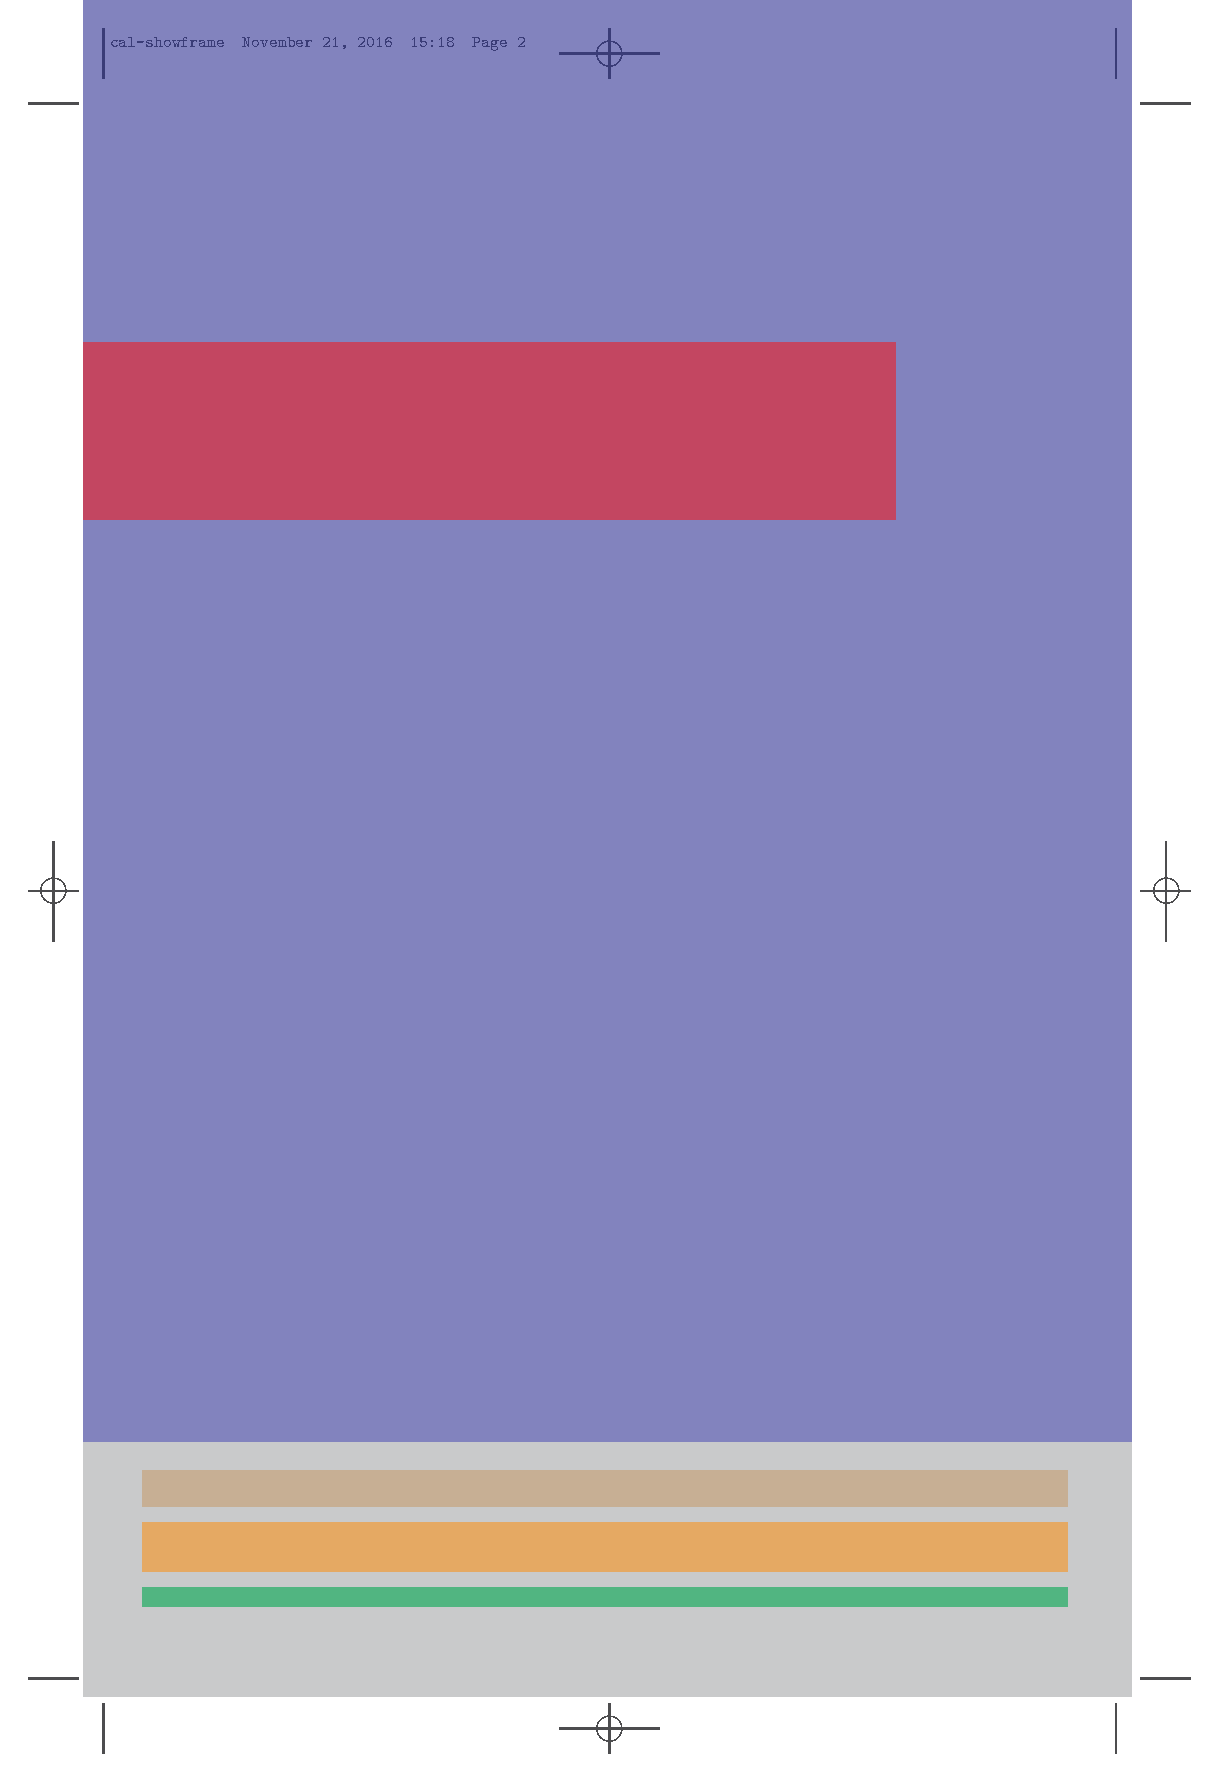
\includegraphics[width=6.12cm]{cal-showframe-02}%
}

Same as June, but we will set the image to be placed above the calendar, and we
add a transparent background for the quote.

This layout is a good option when the top or the bottom of the photo has to be
cropped, and you can't use the full page aspect ratio for the photo.

\begin{verbatim}
\SetPhoto[bleed=3mm, file={obscure-crop}]{July}

\SetQuote[%
  xOffset=0.5\linewidth - 0.5\paperwidth -3mm,
  yOffset=-20mm,
]{July}{%
\begin{tikzpicture}%
\node [
  fill=white, opacity=0.6, minimum width={\paperwidth + 3mm},
  minimum height=30mm] {};%
\node [] {%
\begin{minipage}{\paperwidth + 3mm}%
\centering
\Large
\color{white}

I shall have less to say,\\
But I shall be gone.

\textit{The Sound of the Trees} by Robert Frost
\end{minipage}%
};
\end{tikzpicture}%
}

\ifshowframe
  \SetCalendar[bg/.style={opacity=0.5}]{July}
\else
  \SetCalendar[bg/.style={opacity=1}]{July}
\fi

\SetEvents{July}{
  if (equals=2018-07-27) [day text={\dejaVuSans\char"263C}];
}{%
\raggedleft
{\dejaVuSans\char"263C} July 27: Mars at Opposition
}
\end{verbatim}

\section{August}
\label{sec:org522c828}

\twocol{%
  \frame{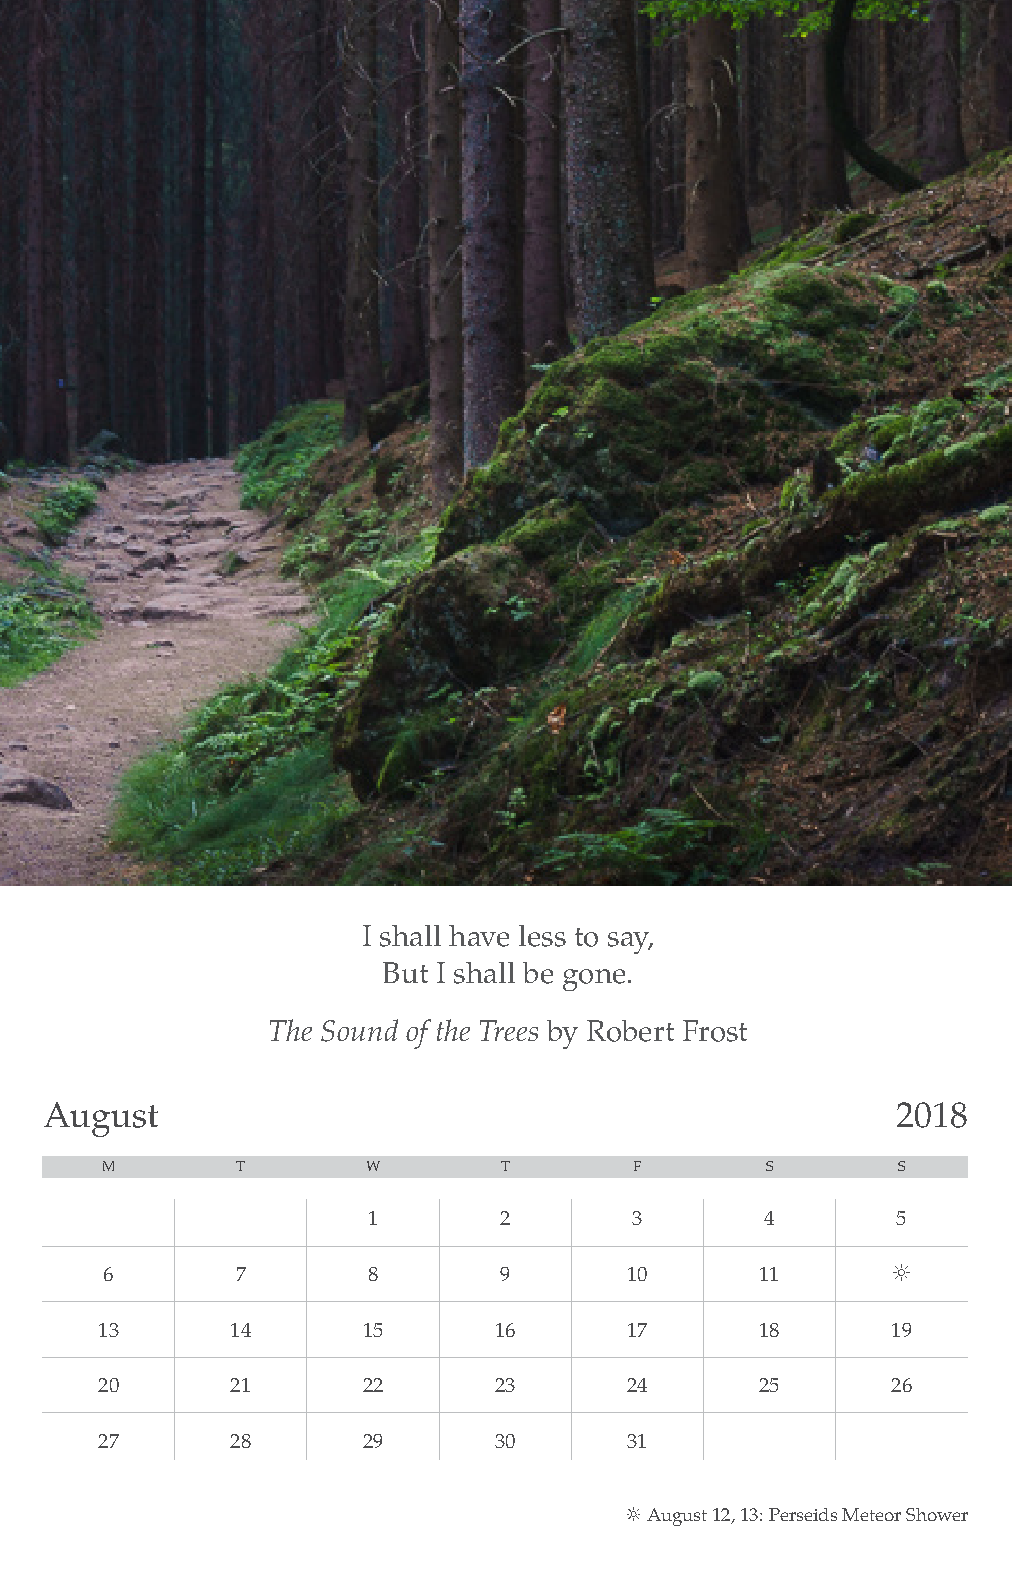
\includegraphics[width=5cm]{cal-plain-03}}%
}{%
  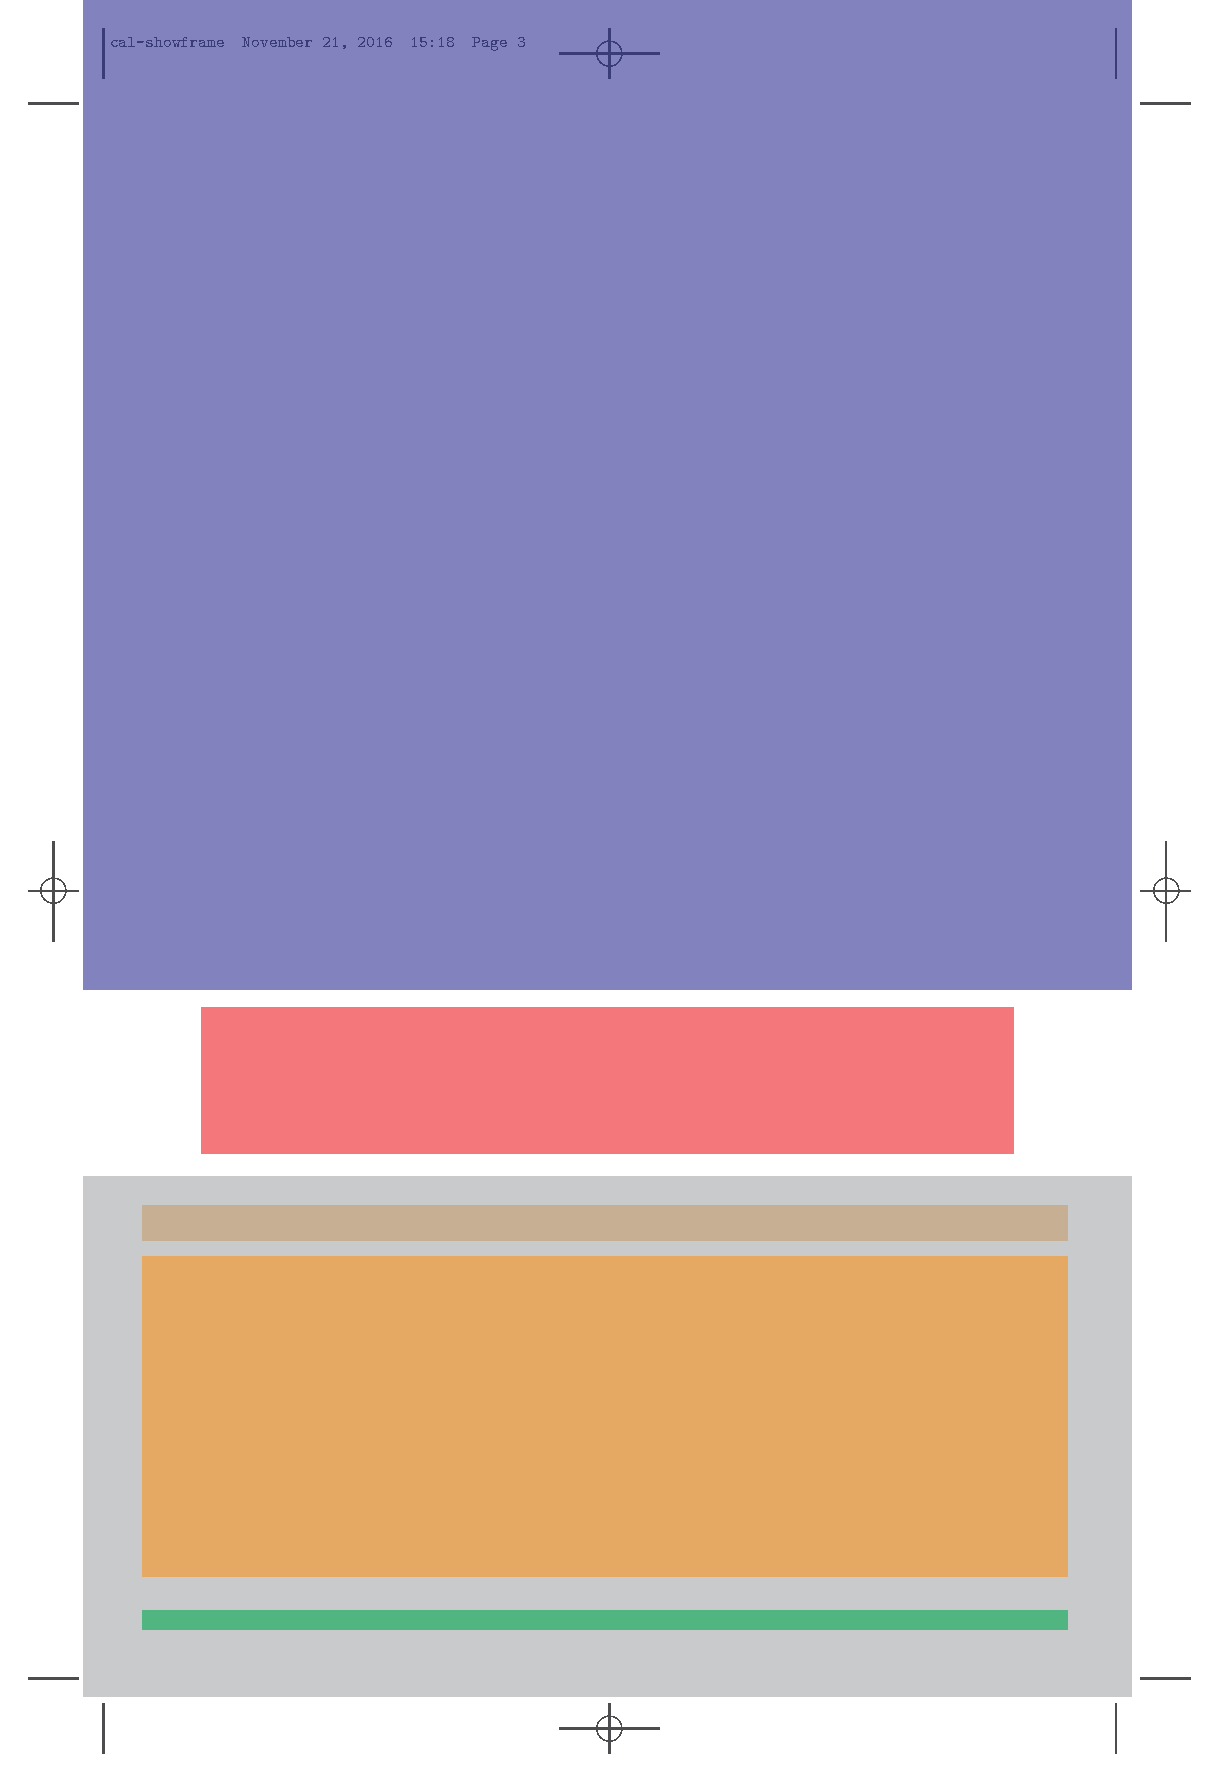
\includegraphics[width=6.12cm]{cal-showframe-03}%
}

This layout works for photos that are horizontal (landscape orientation), scaled
into the bleed margin on three sides.

\begin{verbatim}
\SetPhoto[bleed=3mm, file={obscure-crop}, yOffset=-150mm]{August}

\SetQuote[yOffset=-3mm]{August}{%
\centering
\setlength{\parskip}{10pt}%
\Large
\color{black!80}

I shall have less to say,\\
But I shall be gone.

\textit{The Sound of the Trees} by Robert Frost
}

\ifshowframe
  \SetCalendar[bg/.style={opacity=0.5}]{August}
\else
  \SetCalendar[bg/.style={opacity=1}]{August}
\fi

\SetEvents{August}{
  if (equals=2018-08-12) [day text={\dejaVuSans\char"263C}];
}{%
\raggedleft
{\dejaVuSans\char"263C} August 12, 13: Perseids Meteor Shower
}
\end{verbatim}

End of the preamble.

\begin{verbatim}
\makeatother
\end{verbatim}

\section{The document}
\label{sec:org80f370d}

Typesetting the month pages in the document is now just this much:

\begin{verbatim}
\begin{document}

\MonthPage[layout=full page, put photo=full page]{June}

\MonthPage[layout=full page, put photo=full width above calendar]{July}

\MonthPage[layout=small landscape, put photo=full width]{August}

\end{document}
\end{verbatim}

\clearpage

\chapter{Tutorial: Translations}
\label{sec:org28303a7}

In this tutorial we will produce the same calendar in three languages: Japanese,
English and Hungarian.

We are going to use \texttt{IPAPMincho} font for the Japanese.

\begin{extrafullwidth}

\hfill
\begin{minipage}{0.31\linewidth}
\centering

\frame{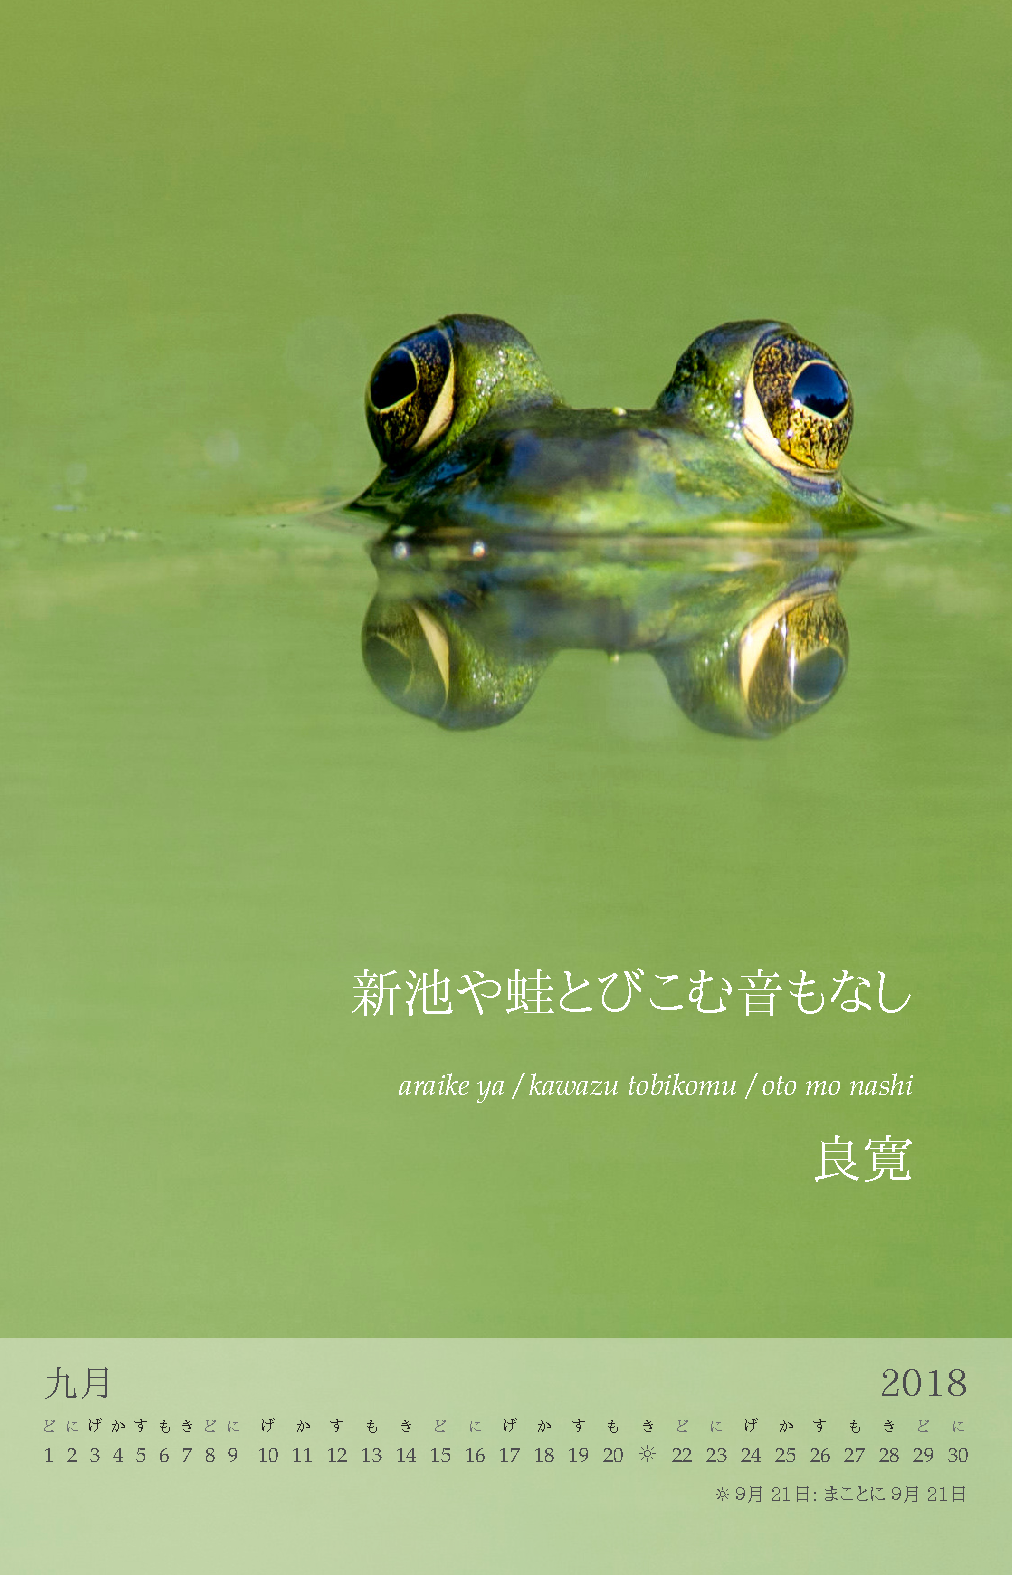
\includegraphics[width=5cm]{./examples/cal-translations-japanese.pdf}}

\end{minipage}%
\begin{minipage}{0.31\linewidth}
\centering

\frame{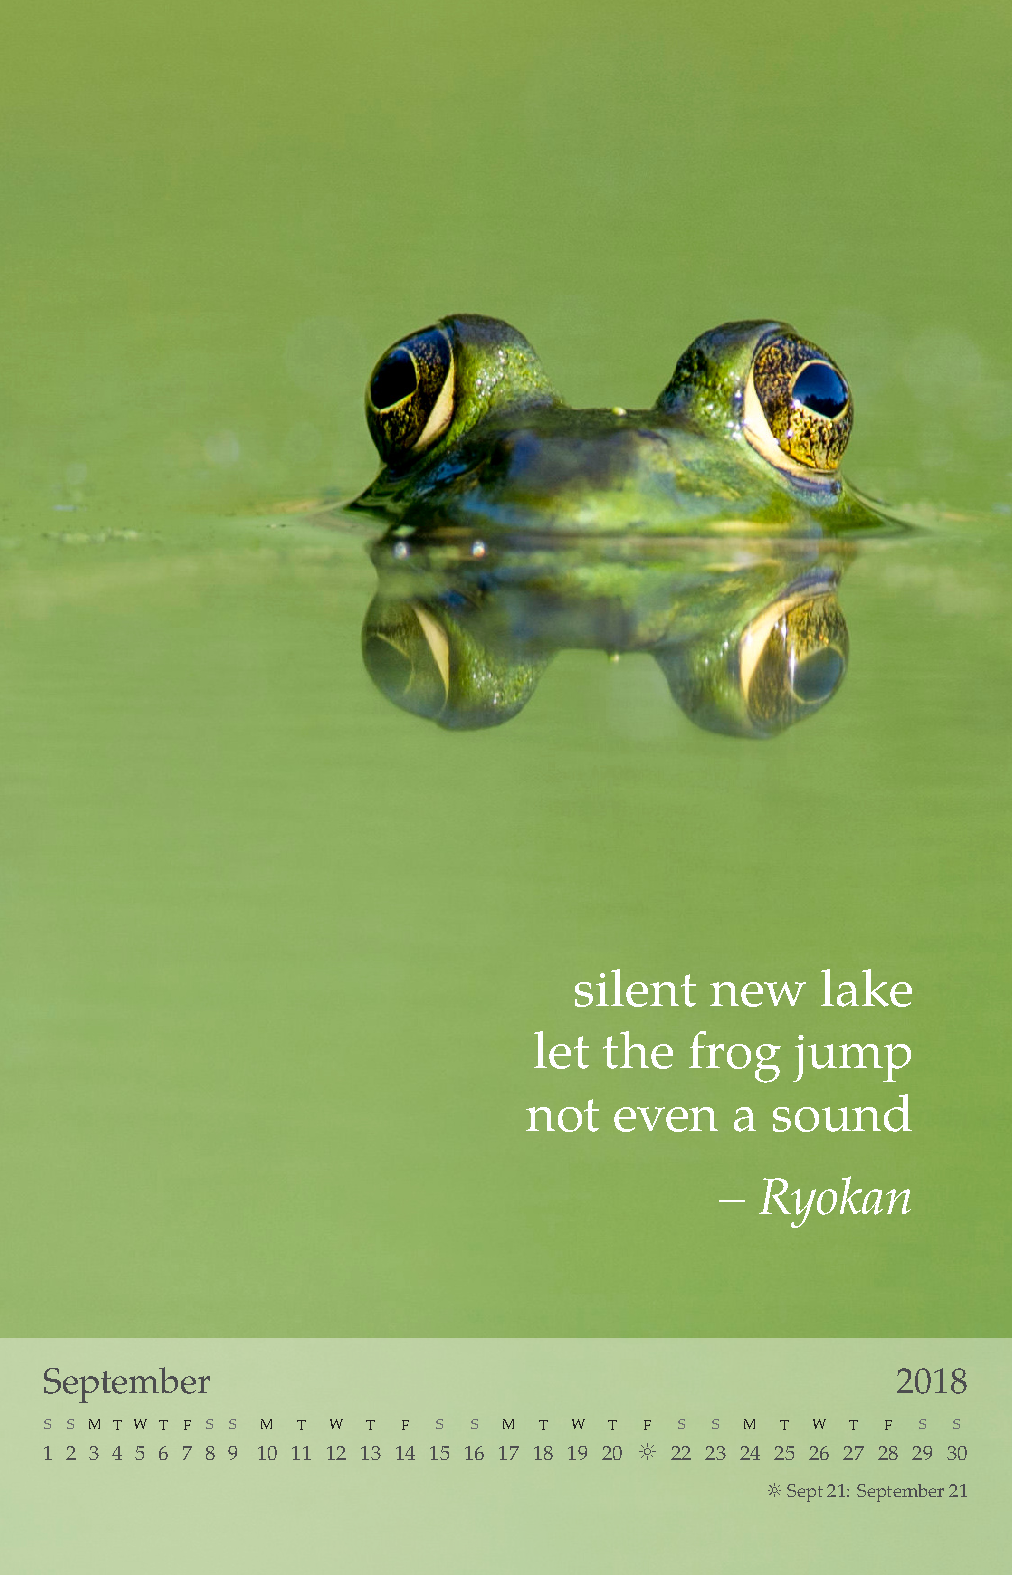
\includegraphics[width=5cm]{./examples/cal-translations-english.pdf}}

\end{minipage}%
\begin{minipage}{0.31\linewidth}
\centering

\frame{
\includegraphics[width=5cm]{./examples/cal-translations-hungarian.pdf}}

\end{minipage}
\hfill\mbox{}

\end{extrafullwidth}

\section{Files}
\label{sec:orga8965a9}

The main document files:

\begin{verbatim}
cal-translations-japanese.tex
cal-translations-english.tex
cal-translations-hungarian.tex
\end{verbatim}

Fonts, formatting settings, etc.:

\begin{verbatim}
local-japanese.sty
local-english.sty
local-hungarian.sty
\end{verbatim}

Translation text input:

\begin{verbatim}
frog-japanese.tex
frog-english.tex
frog-hungarian.tex
\end{verbatim}

Setup month pages (same across translations):

\begin{verbatim}
frog.tex
\end{verbatim}

\section{Translations setup}
\label{sec:org2adcd24}

Create the \texttt{frog-english.tex} file and use the \texttt{\textbackslash{}SetTxt\{ key \}\{ content \}}
command to set text content for translation keys.

\texttt{frog-japanese.tex}

\begin{verbatim}
\SetTxt{September Quote}{%
{\mincho 新池や蛙とびこむ音もなし}

{\Large\textit{araike ya / kawazu tobikomu / oto mo nashi}}

{\mincho 良寛}%
}

\newcommand\SeptMarks{%
  if (equals=2018-09-21)
    [day text={\dejaVuSans\char"263C}];% U+263C white sun with rays
}

\SetTxt{Sept Events}{%
{\dejaVuSans\char"263C} {\mincho 9月 21日: まことに 9月 21日}
}
\end{verbatim}

\texttt{frog-english.tex}

\begin{verbatim}
\SetTxt{September Quote}{%
silent new lake\\
let the frog jump\\
not even a sound

\textit{-- Ryokan}%
}

\newcommand\SeptMarks{%
  if (equals=2018-09-21)
    [day text={\dejaVuSans\char"263C}];% U+263C white sun with rays
}

\SetTxt{Sept Events}{%
{\dejaVuSans\char"263C} Sept 21: September 21
}
\end{verbatim}

\texttt{frog-hungarian.tex}

\begin{verbatim}
\SetTxt{September Quote}{%
hallgat az új tó\\
ugorhat béka belé\\
vize se csobban

\textit{-- Rjókan}%
}

\newcommand\SeptMarks{%
  if (equals=2018-09-21)
    [day text={\dejaVuSans\char"263C}];% U+263C white sun with rays
}

\SetTxt{Sept Events}{%
{\dejaVuSans\char"263C} Szept 21: Szeptember 21
}
\end{verbatim}

\textbf{NOTE:} Using \texttt{\textbackslash{}SetTxt\{\}} to store values intended as tikz marks on the calendar
will not work. The \texttt{\textbackslash{}txt\{\}} command will be the value of \texttt{\textbackslash{}@eventmarks} and tikz
can't resolve it there.

Put the calendar marks in a command instead, as above with \texttt{\textbackslash{}SeptMarks}.

\begin{verbatim}
\calendar (cal#1)
  [alnitak, dates=\CalendarYear-#1-01 to \CalendarYear-#1-last]
  \@eventmarks;%
\end{verbatim}

\begin{verbatim}
% NOTE This code below will not work.
% Put the calendar marks in a command instead.

\SetTxt{Sept Marks}{%
  if (equals=2018-09-21)
    [day text={\dejaVuSans\char"263C}];% U+263C white sun with rays
}

% ...

\SetEvents{September}{%
\txt{Sept Marks}
}{%
\raggedleft
\txt{Sept Events}
}
\end{verbatim}

\section{Document setup}
\label{sec:org736afc3}

Load the documentclass. We are setting the \texttt{translations} option to define the
file where translation keys are set. This file is loaded by the documentclass as
an \texttt{\textbackslash{}input}.

\texttt{cal-translations-japanese.tex}

\begin{verbatim}
\documentclass[
  year = 2018,
  language = japanese,
  translationsInputFile = frog-japanese.tex,
  imageFolder = ./photos/,
]{wallcalendar}

\usepackage{local-japanese}

% Content is the same across translations

\makeatletter

\SetPhoto[bleed=3mm, file={frog-crop}]{September}

\SetQuote[xOffset=0pt, yOffset=-140mm]{September}{%
\raggedleft\setlength{\parskip}{10pt}\HUGE\color{white}%
\txt{September Quote}%
}

\SetCalendar[bg/.style={opacity=0.4}]{September}

\SetEvents{September}{%
\SeptMarks%
}{%
\raggedleft
\txt{Sept Events}
}

\makeatother


\begin{document}

% Just one month
\MonthPage[layout=full page, put photo=full page]{September}

\end{document}
\end{verbatim}

\texttt{local-japanese.sty}

\begin{verbatim}
\ProvidesPackage{local-japanese}

\usepackage{fontspec}
\defaultfontfeatures{Ligatures={TeX}}
\setmainfont{TeX Gyre Pagella}
\newfontfamily\dejaVuSans{DejaVu Sans}
% Japanese font
\newfontfamily\mincho{IPAPMincho}

% Renew formatting hooks to use the \mincho font
\renewcommand\fullPageFmt{%
  \renewcommand*\monthFmt{\LARGE\mincho}%
  \renewcommand*\yearFmt{\LARGE\mincho}%
  \renewcommand*\dayLetterColor{}%
  \renewcommand*\dayLetterFmt{\tiny\mincho}%
  \renewcommand*\dayTextFmt{\small}%
  \renewcommand*\quoteFmt{}%
  \renewcommand*\headingFmt{\centering}%
  \renewcommand*\calendarFmt{\centering}%
  \renewcommand*\eventsFmt{%
   \setlength{\parindent}{0pt}\raggedleft\footnotesize%
  }%
}
\end{verbatim}

\texttt{cal-translations-english.tex}

\begin{verbatim}
\documentclass[
  year = 2018,
  language = english,
  translationsInputFile = frog-english.tex,
  imageFolder = ./photos/,
]{wallcalendar}

\usepackage{local-english}


\makeatletter

\SetPhoto[bleed=3mm, file={frog-crop}]{September}

\SetQuote[xOffset=0pt, yOffset=-140mm]{September}{%
\raggedleft\setlength{\parskip}{10pt}\HUGE\color{white}%
\txt{September Quote}%
}

\SetCalendar[bg/.style={opacity=0.4}]{September}

\SetEvents{September}{%
\SeptMarks%
}{%
\raggedleft
\txt{Sept Events}
}

\makeatother


\begin{document}

\MonthPage[layout=full page, put photo=full page]{September}

\end{document}
\end{verbatim}

\texttt{local-english.sty}

\begin{verbatim}
\ProvidesPackage{local-english}

\usepackage{fontspec}
\defaultfontfeatures{Ligatures={TeX}}
\setmainfont{TeX Gyre Pagella}
\newfontfamily\dejaVuSans{DejaVu Sans}
\end{verbatim}

\texttt{cal-translations-hungarian.tex}

\begin{verbatim}
\documentclass[
  year = 2018,
  language = hungarian,
  translationsInputFile = frog-hungarian.tex,
  imageFolder = ./photos/,
]{wallcalendar}

\usepackage{local-hungarian}


\makeatletter

\SetPhoto[bleed=3mm, file={frog-crop}]{September}

\SetQuote[xOffset=0pt, yOffset=-140mm]{September}{%
\raggedleft\setlength{\parskip}{10pt}\HUGE\color{white}%
\txt{September Quote}%
}

\SetCalendar[bg/.style={opacity=0.4}]{September}

\SetEvents{September}{%
\SeptMarks%
}{%
\raggedleft
\txt{Sept Events}
}

\makeatother


\begin{document}

\MonthPage[layout=full page, put photo=full page]{September}

\end{document}
\end{verbatim}

\texttt{local-hungarian.sty}

\begin{verbatim}
\ProvidesPackage{local-hungarian}

\usepackage{fontspec}
\defaultfontfeatures{Ligatures={TeX}}
\setmainfont{TeX Gyre Pagella}
\newfontfamily\dejaVuSans{DejaVu Sans}
\end{verbatim}

\texttt{frog.tex}

\begin{verbatim}
\makeatletter

\SetPhoto[bleed=3mm, file={frog-crop}]{September}
\end{verbatim}

Use the \texttt{\textbackslash{}txt\{ key \}} command to load text from translation keys:

\begin{verbatim}
\SetQuote[xOffset=0pt, yOffset=-140mm]{September}{%
\raggedleft\setlength{\parskip}{10pt}\HUGE\color{white}%
\txt{September Quote}%
}
\end{verbatim}

Calendar settings for the month, using \texttt{\textbackslash{}txt} to access translated parts.

\begin{verbatim}
\SetCalendar[bg/.style={opacity=0.4}]{September}

\SetEvents{September}{%
\SeptMarks%
}{%
\raggedleft
\txt{Sept Events}
}

\makeatother
\end{verbatim}

\clearpage

\chapter{Tutorial: Load Events from CSV}
\label{sec:org12d351e}

\begin{fullwidth}
\begin{minipage}{\linewidth}
\centering

\frame{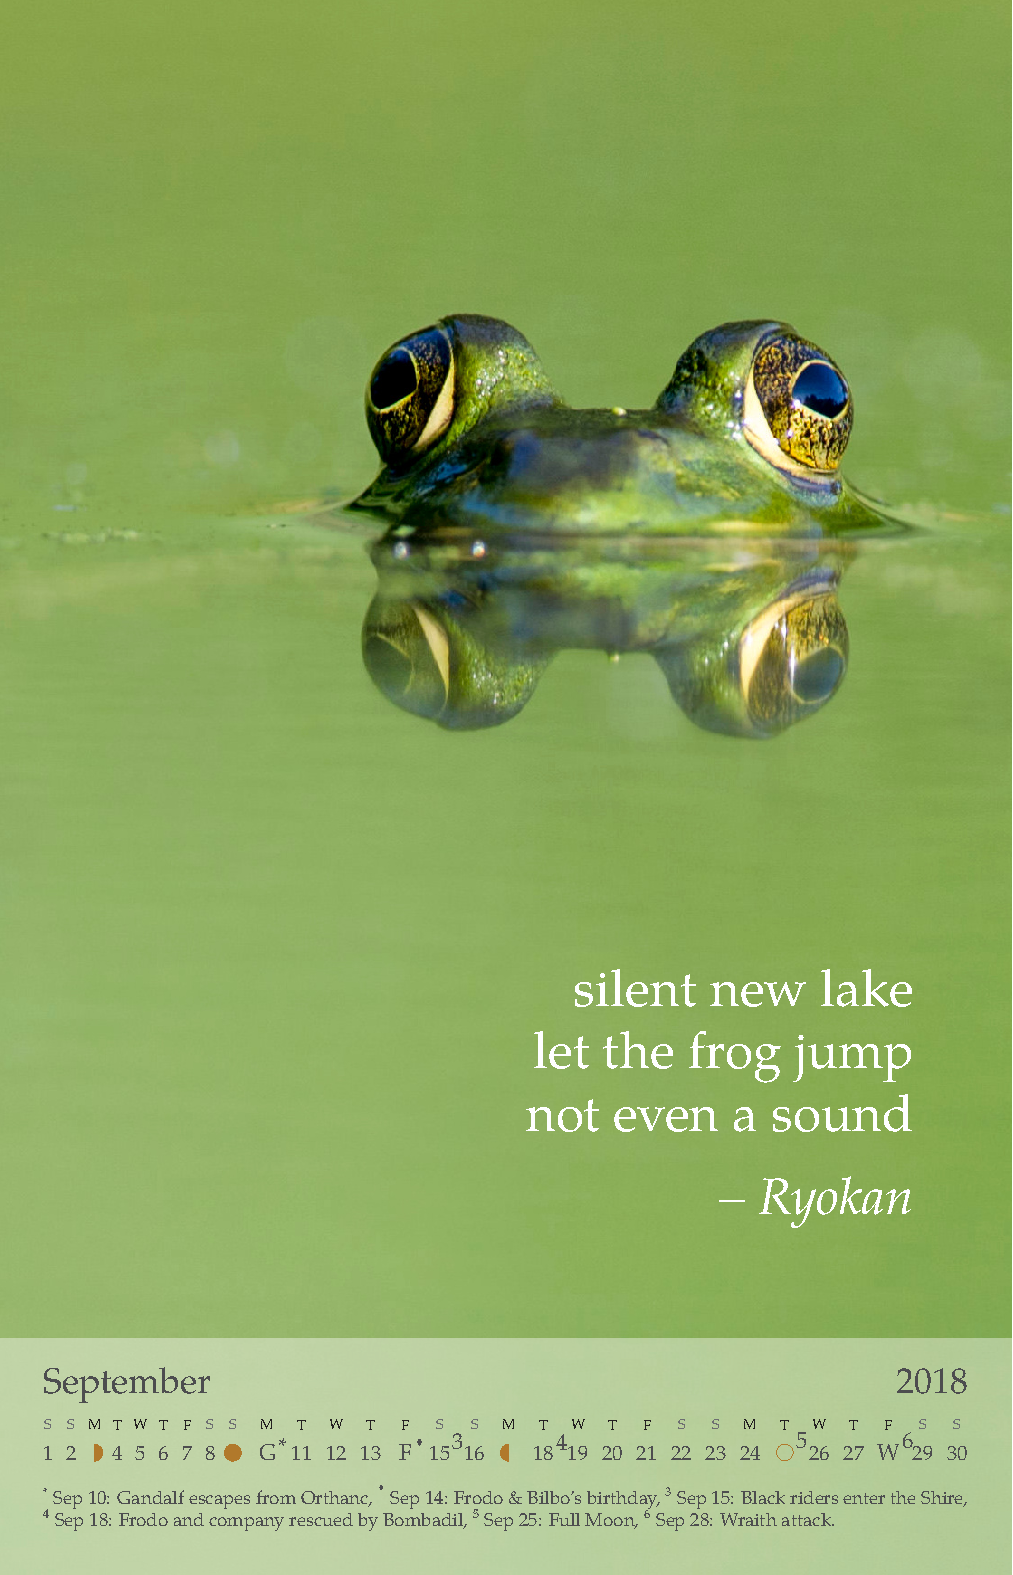
\includegraphics[width=\linewidth, clip, trim=0pt 0pt 0pt 22cm]{./examples/cal-marks.pdf}}

\end{minipage}%
\end{fullwidth}

\section{CSV files}
\label{sec:orgba9e3f8}

Events in the CSV should be already sorted by date.

If you are using more than one CSV, put all events with notes (i.e. indexed
entries) in the same CSV. The index number of the mark is taken from the row
number in the CSV, so a second CSV with notes would start the count from 1
again.

We're going to use the following csv files, see in the \texttt{./doc/examples/data/} folder.

\texttt{holidays.csv}

\texttt{moonphases.csv}

\texttt{mark\_defaults.csv}

\section{Event formatting}
\label{sec:orgbf5aa37}

You can format the event output by setting the \texttt{format cmd} key:

\begin{verbatim}
\parseMonthEvents[%
  format cmd = {%
    \textsuperscript{\eMark}~\eMonthShort~\eDay:\space%
    \eNote\ifnumless{\eIdx}{\eMaxIdx}{,\space}{.}%
  },
]%
\end{verbatim}

Or define a Lua formatting function and set it with the \texttt{format func} key:

\texttt{helpers.lua}

\begin{verbatim}
function eventFmtCustom(idx, max_idx, event, event_date, mark)
  local d = event_date
  tex.sprint(string.format(
    "\\textsuperscript{%s} & %s %s: & %s \\\\",
    mark.symbol, d:fmt("%b"), d:getday(), event.note
  ))
end
\end{verbatim}

\begin{verbatim}
\parseMonthEvents[format func = eventFmtCustom]%
\end{verbatim}

\section{Document setup}
\label{sec:orgb56123b}

\texttt{cal-marks.tex}

\begin{verbatim}
\documentclass[
  year = 2018,
  eventsCsv = ./data/holidays.csv,
  markDefaultsCsv = ./data/mark_defaults.csv,
  imageFolder = ./photos/,
]{wallcalendar}

\makeatletter

\colorlet{mooncolor}{darkgold}

\usepackage{fontspec}
\defaultfontfeatures{Ligatures={TeX}}
\setmainfont{TeX Gyre Pagella}
\newfontfamily\dejaVuSans{DejaVu Sans}

\SetPhoto[bleed=3mm, file={frog-crop}]{September}

\SetQuote[xOffset=0pt, yOffset=-140mm]{September}{%
\raggedleft\setlength{\parskip}{10pt}\HUGE\color{white}%
silent new lake\\
let the frog jump\\
not even a sound

\textit{-- Ryokan}%
}

\SetCalendar[bg/.style={opacity=0.4}]{September}

\SetEvents{September}{%
\parseMonthMarksDayTextUsing{./data/moonphases.csv}%
\parseMonthMarksDayText%
\parseMonthMarksNote%
}{%
\raggedright
\parseMonthEvents[%
  format cmd = {%
    \textsuperscript{\eMark}~\eMonthShort~\eDay:\space%
    \eNote\ifnumless{\eIdx}{\eMaxIdx}{,\space}{.}%
   },
]%
}

\makeatother

\begin{document}

\MonthPage[layout=full page, put photo=full page]{September}

\end{document}
\end{verbatim}

\clearpage

\chapter{Example: Year Planner Page}
\label{sec:org24663e1}

\begin{fullwidth}
\begin{minipage}{0.31\linewidth}
\centering

\frame{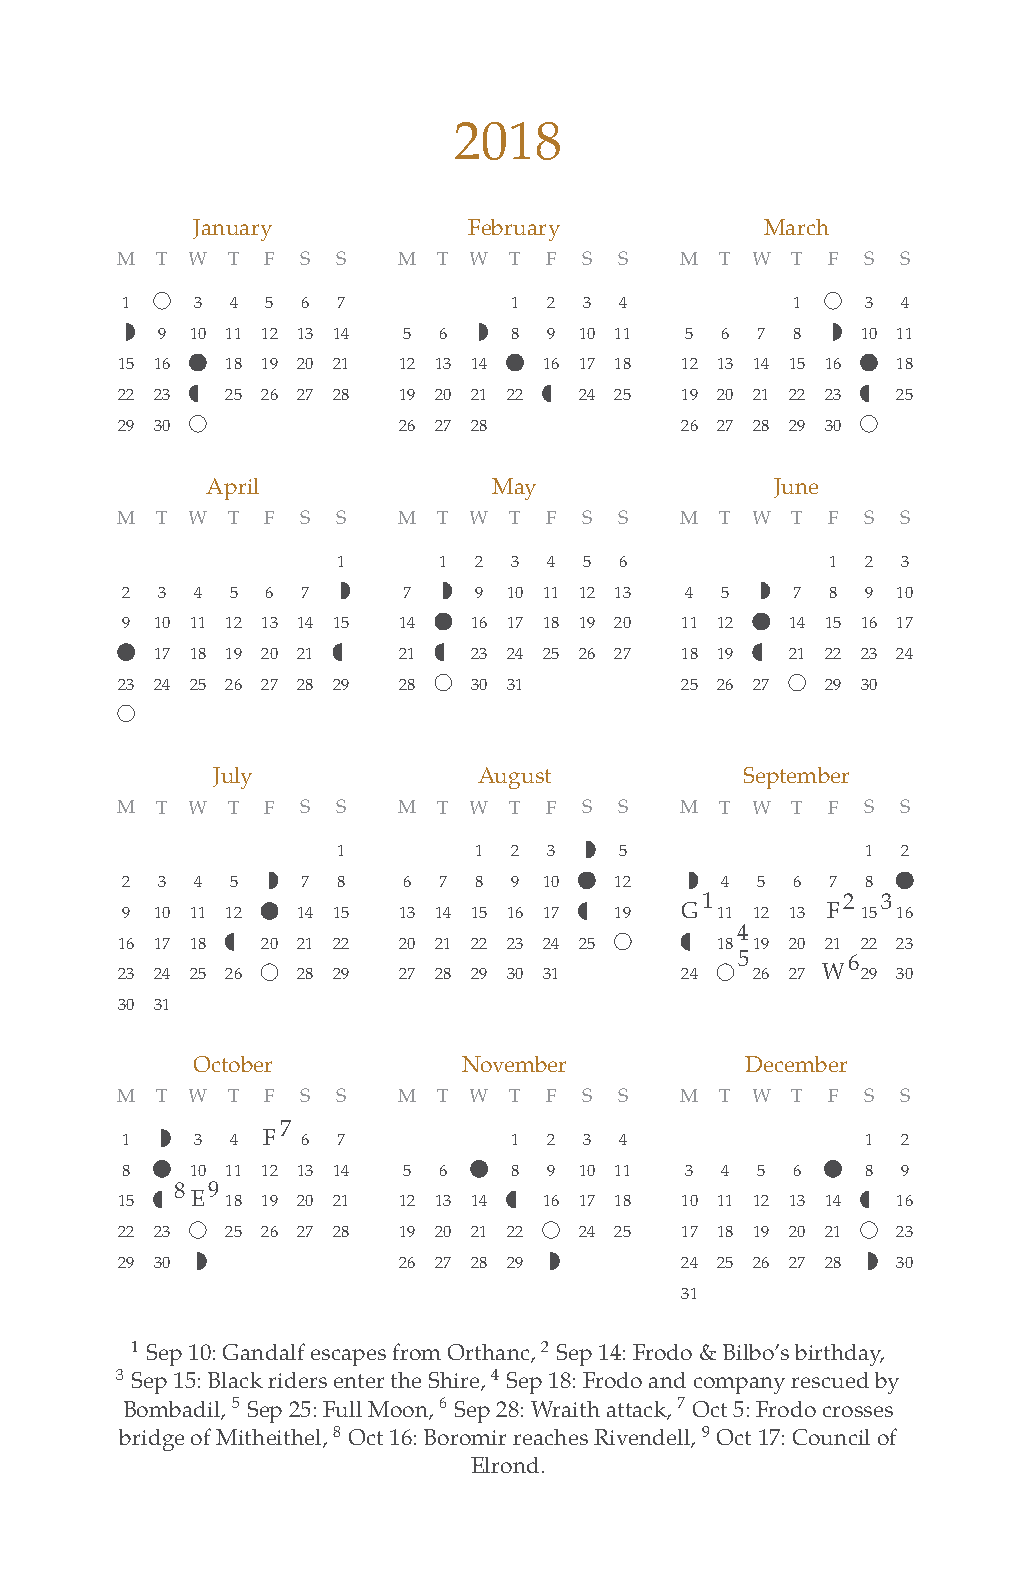
\includegraphics[width=5cm]{./examples/cal-year-planner.pdf}}

\end{minipage}%
\end{fullwidth}

\section{Document setup}
\label{sec:org85fac7e}

\texttt{cal-year-planner.tex}

\begin{verbatim}
\documentclass[
  year = 2018,
  eventsCsv = ./data/holidays.csv,
  markDefaultsCsv = ./data/mark_defaults.csv,
  imageFolder = ./photos/,
]{wallcalendar}

\makeatletter

\usepackage{fontspec}
\defaultfontfeatures{Ligatures={TeX}}
\setmainfont{TeX Gyre Pagella}
\newfontfamily\dejaVuSans{DejaVu Sans}

% Use two CSV files for day text input to include the moon phases
\renewcommand\@wall@plm[1]{%
\luadirect{
require("wallcalendar-helpers.lua")
monthMarksDayText(\luastring{#1}, nil, \luastring{\plannerMarksDayTextCSV})
monthMarksDayText(\luastring{#1}, nil, \luastring{./data/moonphases.csv})
tex.sprint(';')
}}
\end{verbatim}

\section{\textbackslash YearPlannerPage}
\label{sec:org0124cf4}

\begin{verbatim}
\newcommand\plannerYearFmt{\fontsize{26}{26}\selectfont\color{orangegold}}

\newlength\plannerNotesSep
\setlength{\plannerNotesSep}{3mm}

\newcommand\preYearPlannerPageHook{%
  \setlength{\markNumberAbove}{-9pt}%
  \setlength{\markNumberRight}{-6pt}%
  \setlength{\markDayTextAbove}{-11pt}%
  \setlength{\markDayTextRight}{-6pt}%
}

\newcommand\postYearPlannerPageHook{%
  \setlength{\markNumberAbove}{-10pt}%
  \setlength{\markNumberRight}{-3pt}%
  \setlength{\markDayTextAbove}{-10pt}%
  \setlength{\markDayTextRight}{-3pt}%
}

\newcommand\printPlannerTitle{\plannerYearFmt \CalendarYear}

\newcommand\YearPlannerPage{%
\newpage
\ifvarnishmask
\mbox{}
\else
\preYearPlannerPageHook
{\centering

{\printPlannerTitle}

\vspace*{7mm}

\YearPlannerPortrait

\vspace*{\plannerNotesSep}

\plannerEvents

}
\postYearPlannerPageHook

\fi
}

\makeatother
\end{verbatim}

\section{Use it}
\label{sec:org70f504f}

\begin{verbatim}
\begin{document}

\YearPlannerPage

\end{document}
\end{verbatim}

\clearpage

\chapter{Example: Photo Thumbnails Page}
\label{sec:org0431559}

\begin{fullwidth}
\begin{minipage}{0.31\linewidth}
\centering

\frame{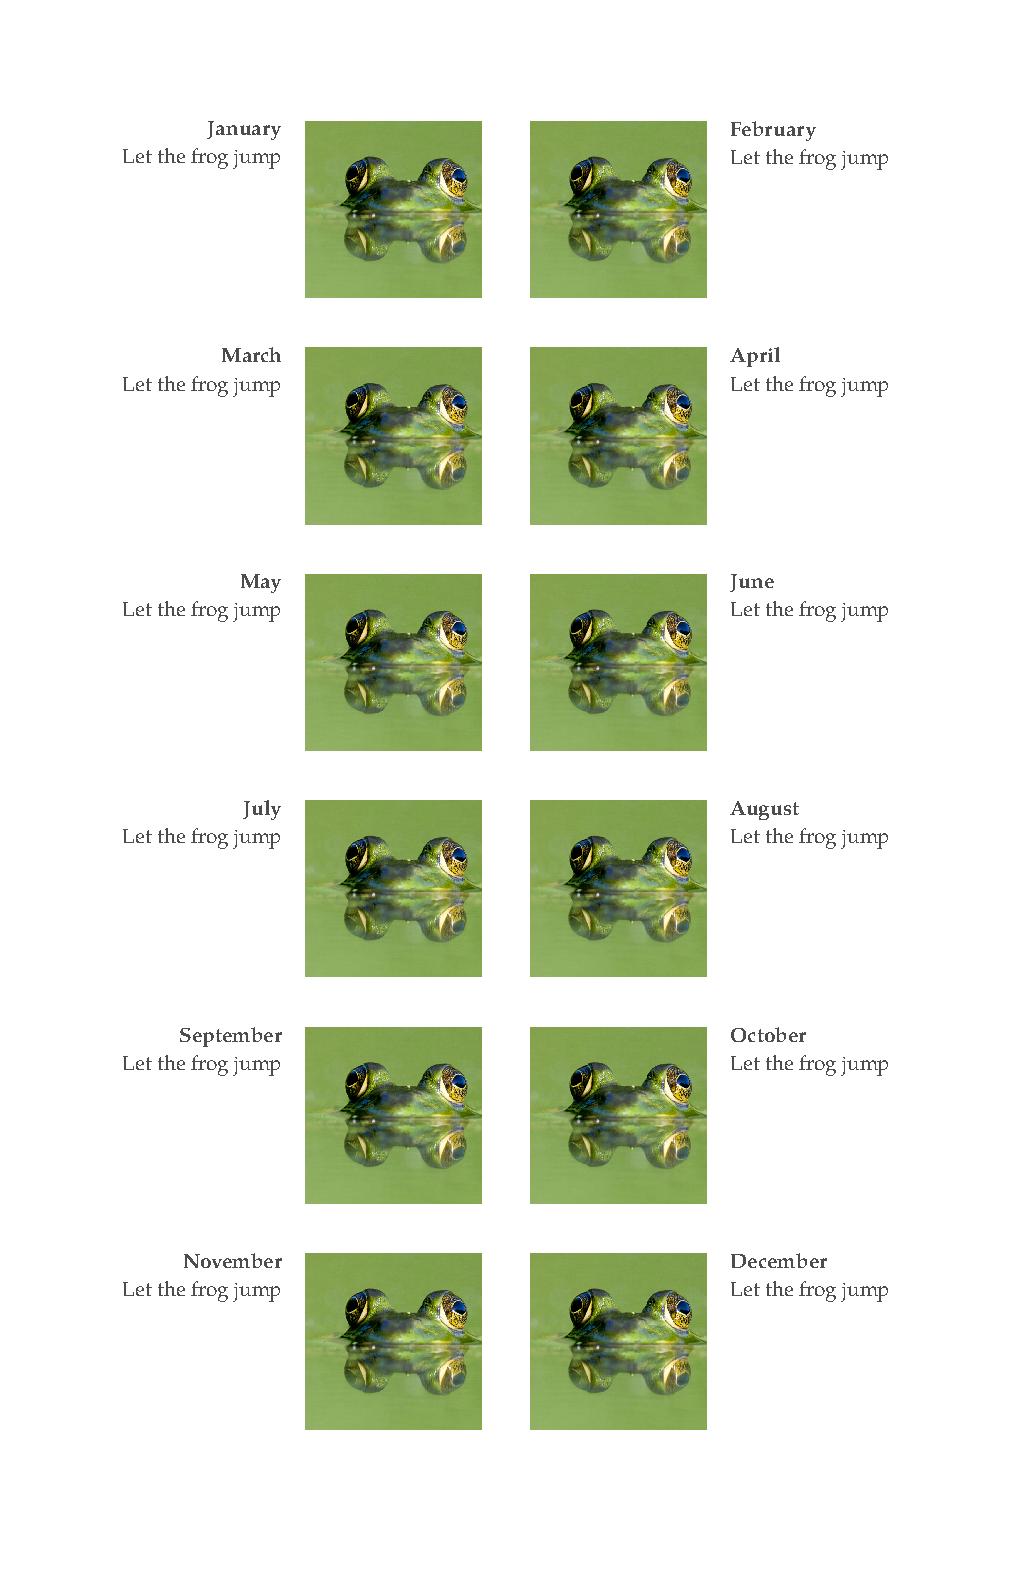
\includegraphics[width=5cm]{./examples/cal-thumbnails.pdf}}

\end{minipage}%
\end{fullwidth}

\section{Document setup}
\label{sec:orgc4970c9}

\texttt{cal-thumbnails.tex}

\begin{verbatim}
\documentclass[
  year = 2018,
  imageFolder = ./photos/,
]{wallcalendar}

\makeatletter

\usepackage{fontspec}
\defaultfontfeatures{Ligatures={TeX}}
\setmainfont{TeX Gyre Pagella}
\newfontfamily\dejaVuSans{DejaVu Sans}

\newlength\@wall@tmp@a
\newlength\@wall@tmp@b
\end{verbatim}

\section{\textbackslash ThumbWithCaptionLeftSide}
\label{sec:orge74d943}

Typesets the photo thumb image with its caption text on the left side.

\begin{verbatim}
\ThumbWithCaptionLeftSide{January}
\end{verbatim}

\begin{verbatim}
\newlength\@wall@thumbWidth
\newlength\@wall@thumbHeight
\newlength\@wall@thumbCaptionWidth
\setlength{\@wall@thumbWidth}{0.1749\calPaperWidth}% 30mm at the 6.75in page width, 0.1749 = 1/5.715
\setlength{\@wall@thumbHeight}{\@wall@thumbWidth}
\setlength{\@wall@thumbCaptionWidth}{0.2333\calPaperWidth}% 40mm at 6.75in page width

\newcommand\thumbFmt{}
\newcommand\thumbMonthFmt{\fontsize{10}{13}\selectfont\bfseries}
\newcommand\thumbCaptionFmt{\fontsize{10}{13}\selectfont}

\def\@wall@thumbFile{}
\def\@wall@photoCaption{}

\newcommand\ThumbWithCaptionLeftSide[1]{%
\pgfkeys{/Photo/#1/thumbFile/.get=\@wall@thumbFile}%
\ifx\@wall@thumbFile\empty
  \pgfkeys{/Photo/#1/file/.get=\@wall@thumbFile}%
\fi
\pgfkeys{/Photo/#1/caption/.get=\@wall@photoCaption}%
% Thumbnail caption
\ifvarnishmask%
\hspace*{\@wall@thumbWidth}
\else%
\begin{minipage}[b][\@wall@thumbHeight][t]{\@wall@thumbCaptionWidth}%
\raggedleft
\thumbFmt
{\thumbMonthFmt \@tr@monthNumName{\monthToNum{#1}}}\par
{\thumbCaptionFmt \@wall@photoCaption}%
\end{minipage}%
\fi%
\hspace*{3mm}
% Thumbnail photo
\begin{minipage}[b][\@wall@thumbHeight]{\@wall@thumbWidth}%
% FIXME placeholder
%\placeholder{%
\includegraphics[ keepaspectratio, height=\@wall@thumbHeight ]{\@wall@thumbFile}%
%}%
\end{minipage}%
}
\end{verbatim}

\section{\textbackslash ThumbWithCaptionRightSide}
\label{sec:org7af4bd6}

Typesets the photo thumb image with its caption text on the right side.

\begin{verbatim}
\ThumbWithCaptionRightSide{January}
\end{verbatim}

\begin{verbatim}
\newcommand\ThumbWithCaptionRightSide[1]{%
\pgfkeys{/Photo/#1/thumbFile/.get=\@wall@thumbFile}%
\ifx\@wall@thumbFile\empty
  \pgfkeys{/Photo/#1/file/.get=\@wall@thumbFile}%
\fi
\pgfkeys{/Photo/#1/caption/.get=\@wall@photoCaption}%
% Thumbnail photo
\begin{minipage}[b][\@wall@thumbHeight]{\@wall@thumbWidth}%
% FIXME placeholder
%\placeholder{%
\includegraphics[ keepaspectratio, height=\@wall@thumbHeight ]{\@wall@thumbFile}%
%}%
\end{minipage}%
\hspace*{3mm}
% Thumbnail caption
\ifvarnishmask%
\hspace*{\@wall@thumbWidth}
\else%
\begin{minipage}[b][\@wall@thumbHeight][t]{\@wall@thumbCaptionWidth}%
\raggedright
\thumbFmt
{\thumbMonthFmt \@tr@monthNumName{\monthToNum{#1}}}\par
{\thumbCaptionFmt \@wall@photoCaption}%
\end{minipage}%
\fi%
}
\end{verbatim}

\section{\textbackslash ThumbsPage}
\label{sec:org9571a13}

\begin{verbatim}
\newlength{\thumbColumnWidth}
\newlength{\thumbColumnHeight}
\newlength{\thumbSep}
\newlength{\@t@a}
\newlength{\@t@b}

% vertical spacing
\setlength{\@t@a}{0.2\textheight}

% horizontal spacing
\setlength{\@t@b}{0.2\@wall@thumbCaptionWidth}% 8mm at 40mm caption width

\ifdimcomp{\@t@a}{<}{\@t@b}{
  \setlength{\thumbSep}{\@t@a}
}{
  \setlength{\thumbSep}{\@t@b}
}

\setlength{\thumbColumnWidth}{0.5\calPaperWidth - \thumbSep}
\setlength{\thumbColumnHeight}{\textheight}

\newcommand\ThumbsPage{%
\clearpage

\hspace*{-\@wall@leftMargin}%
\hspace*{-1pt}% small correction, space gets in somewhere
% Wrap
\begin{minipage}[t][\thumbColumnHeight]{\calPaperWidth}%
\centering%
\setlength{\parindent}{0pt}%
\setlength{\parskip}{0pt}%

% NOTE: multicols will not \vfill
% Left Column
\begin{minipage}[t][\thumbColumnHeight]{\thumbColumnWidth}%
\raggedleft

\ThumbWithCaptionLeftSide{January}

\vspace*{\thumbSep}

\ThumbWithCaptionLeftSide{March}

\vspace*{\thumbSep}

\ThumbWithCaptionLeftSide{May}

\vspace*{\thumbSep}

\ThumbWithCaptionLeftSide{July}

\vspace*{\thumbSep}

\ThumbWithCaptionLeftSide{September}

\vspace*{\thumbSep}

\ThumbWithCaptionLeftSide{November}

% End of left column
\end{minipage}%
%
\hspace*{\thumbSep}%
%
% Right column
\begin{minipage}[t][\thumbColumnHeight]{\thumbColumnWidth}%
\raggedright

\ThumbWithCaptionRightSide{February}

\vspace*{\thumbSep}

\ThumbWithCaptionRightSide{April}

\vspace*{\thumbSep}

\ThumbWithCaptionRightSide{June}

\vspace*{\thumbSep}

\ThumbWithCaptionRightSide{August}

\vspace*{\thumbSep}

\ThumbWithCaptionRightSide{October}

\vspace*{\thumbSep}

\ThumbWithCaptionRightSide{December}

% End of right column
\end{minipage}%

% End of wrap
\end{minipage}%
}
\end{verbatim}

\section{Setup the photo keys}
\label{sec:org1bdd209}

\begin{verbatim}
\SetPhoto[file={frog-crop}, thumbFile={frog-crop-thumb}, caption={Let the frog jump}]{January}
\SetPhoto[file={frog-crop}, thumbFile={frog-crop-thumb}, caption={Let the frog jump}]{February}
\SetPhoto[file={frog-crop}, thumbFile={frog-crop-thumb}, caption={Let the frog jump}]{March}
\SetPhoto[file={frog-crop}, thumbFile={frog-crop-thumb}, caption={Let the frog jump}]{April}
\SetPhoto[file={frog-crop}, thumbFile={frog-crop-thumb}, caption={Let the frog jump}]{May}
\SetPhoto[file={frog-crop}, thumbFile={frog-crop-thumb}, caption={Let the frog jump}]{June}
\SetPhoto[file={frog-crop}, thumbFile={frog-crop-thumb}, caption={Let the frog jump}]{July}
\SetPhoto[file={frog-crop}, thumbFile={frog-crop-thumb}, caption={Let the frog jump}]{August}
\SetPhoto[file={frog-crop}, thumbFile={frog-crop-thumb}, caption={Let the frog jump}]{September}
\SetPhoto[file={frog-crop}, thumbFile={frog-crop-thumb}, caption={Let the frog jump}]{October}
\SetPhoto[file={frog-crop}, thumbFile={frog-crop-thumb}, caption={Let the frog jump}]{November}
\SetPhoto[file={frog-crop}, thumbFile={frog-crop-thumb}, caption={Let the frog jump}]{December}

\makeatother
\end{verbatim}

\section{Use it}
\label{sec:org23c0fca}

\begin{verbatim}
\begin{document}

\ThumbsPage

\end{document}
\end{verbatim}

\chapter{Documentclass Options}
\label{sec:org5024f18}

\begin{verbatim}
year
\end{verbatim}

\begin{verbatim}
language
\end{verbatim}

\begin{verbatim}
imageFolder
\end{verbatim}

\begin{verbatim}
showframe
\end{verbatim}

\begin{verbatim}
showtrims
\end{verbatim}

\begin{verbatim}
varnishmask
\end{verbatim}

\chapter{User Commands}
\label{sec:org02a2f80}

\begin{verbatim}
\SetPhoto[ options ]{ month }
\end{verbatim}

\begin{verbatim}
\SetQuote[ options ]{ month }{ quote text }
\end{verbatim}

\begin{verbatim}
\SetCalendar[ options ]{ month }
\end{verbatim}

\begin{verbatim}
\SetEvents[ options ]{ month }{ calendar tikz marks }{ events text }
\end{verbatim}

\begin{verbatim}
\MonthPage[ options ]{ month }
\end{verbatim}

\clearpage

\chapter{Page Layout}
\label{sec:org2801ae6}

We will review how the page layout happens when we call \texttt{\textbackslash{}MonthPage}.

Before calling \texttt{\textbackslash{}MonthPage} to typeset a particular month, be sure that the
content for the given month has been already set with \texttt{\textbackslash{}SetPhoto}, \texttt{\textbackslash{}SetQuote},
\texttt{\textbackslash{}SetCalendar} and \texttt{\textbackslash{}SetEvents}.

Then we can typeset that month, for example:

\begin{verbatim}
\MonthPage[layout=full page, put photo=full page]{June}
\end{verbatim}

This will be a full page portrait month with the photo scaled to cover the
entire page with additional bleed on all four sides.

\twocol{%
  \frame{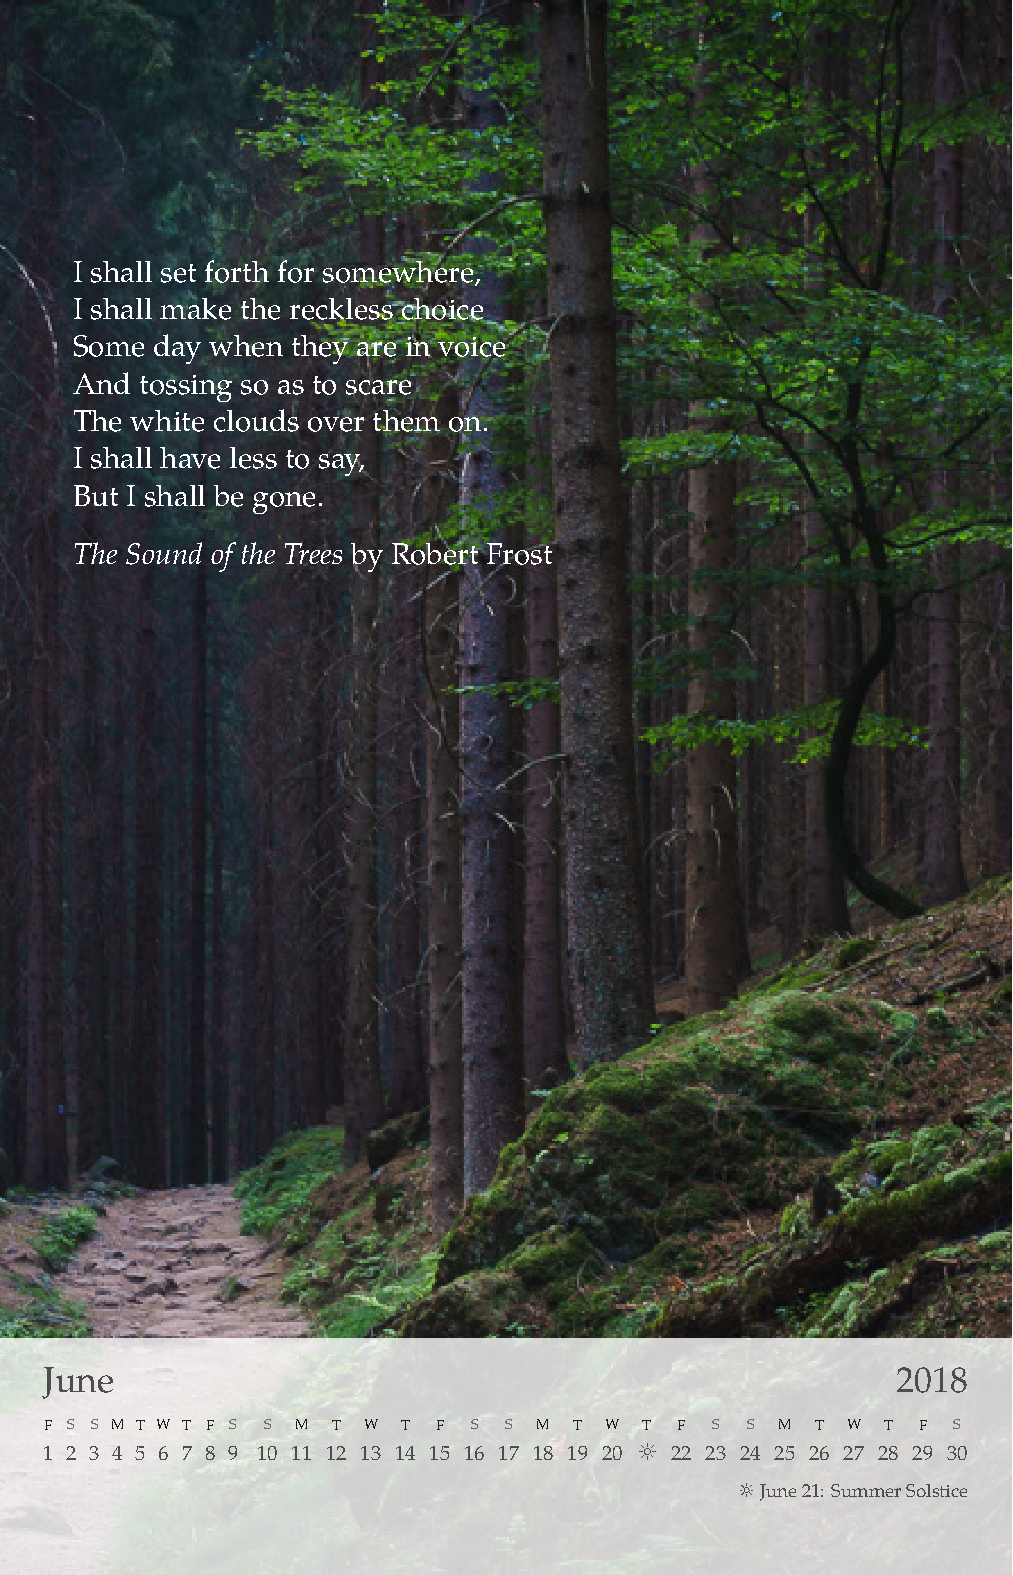
\includegraphics[width=5cm]{cal-plain-01}}%
}{%
  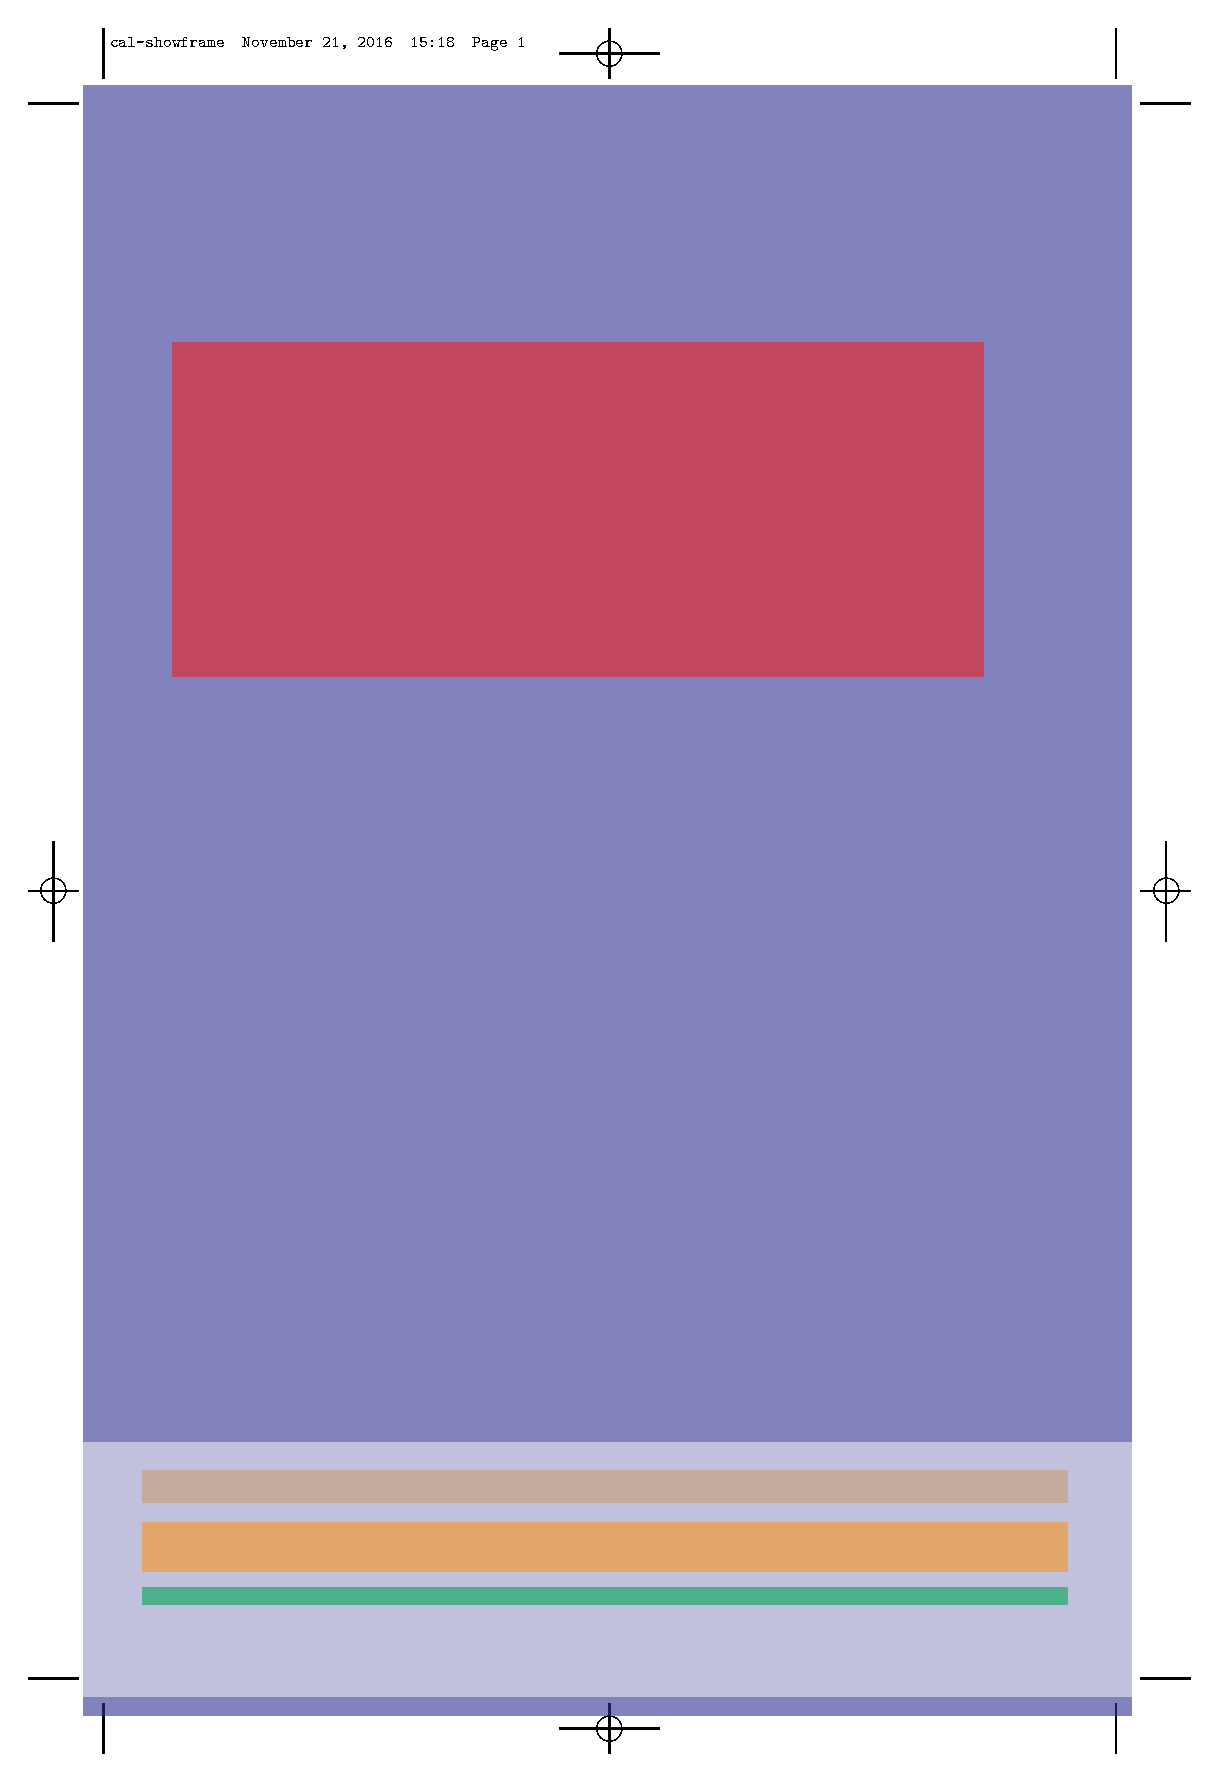
\includegraphics[width=6.12cm]{cal-showframe-01}%
}

The above \texttt{showframe} figure shows the structural elements of the page.

Every layout is implemented by a single handler macro which will deal with all
the typesetting of the given page. The \texttt{full page} key is set to the
\texttt{\textbackslash{}@wall@fullPageLayout} macro by default, and so this gets called.

The layout macro is just a free-style placeholder. It can access the photo,
quote, calendar and events as set earlier, but it is up to the macro to
implement what to do with them.

This is for the convenience of setting the page elements using the same
interface, but being able to execute different layouts for different pages.

The class contains two layout examples. The \texttt{full page} layout is best for
portrait photos that can be scaled to cover the entire page. The \texttt{small
landscape} layout is for landscape photos which can be scaled horizontally,
possibly bleeding into the side margins.

\chapter{Contact}
\label{sec:orgc9e6d1d}

Github: \url{https://github.com/profound-labs/wallcalendar/}

Email: \texttt{Gambhīro Bhikkhu <gambhiro.bhikkhu.85@gmail.com>}
\end{document}
